\chapter{Evaluation Based on Use Cases}\label{chap:applications}
\glsadd{csv}\glsadd{fps}\glsadd{fifo}

\section{Introduction}
\label{sec:app-intro}

We apply the framework of \cref{chap:contribution} to five scenarios and report what the recorded runs measured: a daily urban routine, two shopping centers, an emergency evacuation and a set of directed-flow corridors. All scenarios use the same implementation of a person, schedule parser, movement layer and station model, and they differ only in the schedule file, the map and a small manager that prepares the map. The scenarios show what the rule language can express with little new code, as only Mall B needed a new action, \texttt{Interact}, with its button and gate. We also use them to make preliminary measurements of the waiting at shared resources, of the drift between authored and realized times and of how many people one desktop computer can animate. No test compares the simulated people with real pedestrians, but the runs did expose a number of edge cases, which we report where they affect the numbers. \Cref{sec:app-setup} describes the experimental setup, and \cref{sec:app-dul,sec:app-mall,sec:app-evac,sec:app-validation} evaluate the daily urban life, shopping center, evacuation and directed-flow use cases. \Cref{sec:app-performance} then measures performance and scalability, \cref{sec:app-threats} discusses the threats to validity and \cref{sec:app-summary} concludes the chapter.

\section{Experimental Setup}
\label{sec:app-setup}

\begin{center}
\fbox{\parbox{0.94\textwidth}{\textbf{Time modes.} Every behavioral result in this chapter uses Accurate mode, in which walking and the clock advance together. Visual-mode timings, in which a 100~m walk counts as about 50 simulated minutes, are not valid as timings, and they appear only in the rendered scaling runs of \cref{sec:app-performance}, where only the cost of each frame matters.}}
\end{center}

\subsection{Machine, modes and settings}
\label{sub:app-settings}

All runs used one desktop computer with an AMD Ryzen~7 7800X3D processor (eight cores), an AMD Radeon RX 7900 XTX graphics card (24~GB) and 32~GB of DDR5-6000 memory. The game ran from the Development editor binaries of \gls{ue}~5.4 (\texttt{UnrealEditor.exe -game}) rather than a packaged Shipping build, and the navigation mesh was generated when each level loaded. Behavioral runs used \texttt{-nullrhi}, which skips rendering, and only the scaling runs (\cref{sec:app-performance}) were rendered, in a 1920$\times$1080 window. Vertical synchronization was off in the rendered runs, so the monitor did not cap the frame rate (\cref{tab:flags}). The people are MetaHuman characters with skeletal animation and hair strands. As in the development configuration, \texttt{enableInfrastructureAnalysis} was on in every run, so idle people stopped instead of flocking, queued people waited without a timeout, and a failed path left the person stopped with their reservation (\cref{tab:experiment-settings}). The boids therefore act in only part of these runs, because idle flocking was off and the blend steers scheduled walks but not walks to a reserved station, queued people or the evacuation, where people follow their paths.

Every behavioral run used Accurate mode (\cref{sec:clock-modes}), in which walking and the clock advance by the same simulated time in each frame. The unrendered runs also used the engine's fixed time step (\texttt{-UseFixedTimeStep -FPS=30}), so every frame was exactly one simulated second, regardless of how fast the machine produced frames. A shopping-center run of about three simulated hours therefore took about half a minute, and a Daily Urban Life run about three minutes. To check how much the results depend on that step, we repeated the evacuation and a subset of the shopping-center and Daily Urban Life runs with 0.25 simulated seconds per frame (\texttt{-FPS=120}, \cref{sub:app-step}). The scaling runs measure how many people can be watched interactively, so they were rendered in real time in Visual mode, the mode for viewing. People walk at 200~cm/s by default and at 170 to 230~cm/s in Daily Urban Life. We did not calibrate these speeds, which are faster than the 1.34~m/s of a free pedestrian \citep{weidmann1993transporttechnik}, so in Accurate mode a 100~m walk lasts about 50 simulated seconds, roughly a third less than a real pedestrian would need. Three time-outs do not go through this conversion and still count real seconds (\cref{sec:clock-modes}): the GoTo time-out ends a walk after 90 simulated minutes, the queue time-out after 25, and an exit serves one person every 45 simulated seconds. The queue time-out is unused here, because queued people waited without a time-out, and we note every result that the other two constants affect. An earlier round of runs in Visual mode was superseded by this one for every behavioral result.

The runs used a test branch that adds to the main branch the recorder and the stress test of \cref{app:tooling}, together with four adjustments for steps of one simulated second, in which a person moves about 2~m. The path follower accepts a waypoint that the person has walked past within two frames of travel, and the final walk onto an evacuation slot or into the safe zone is shortened so that the person stops inside the slot window. Needs also advance in simulated minutes, and the movement component substeps every 0.05 simulated seconds so that its ledge checks follow ramps. The same branch also lets the capacity setting match station identifiers, so that it reaches the food counters and tables, keeps the clock running when a run meets its end condition before the export timer fires, so that the mall export is still written, and starts the evacuation summary before people react. The results therefore reflect this branch rather than the main branch alone. The public repository \citep{armada2026repository} holds the framework on its main branch and, beside it, this test branch with its batch scripts and run configurations, while the recorded run files are not public.

Runs start at 07:30 so that the navigation mesh is ready before the first path request, except the evacuation, which starts at the default of 08:00, five minutes before its only rule. The shopping-center runs were capped at 11:20, and most of them ended at about 10:30, when every rule had been consumed and no person was busy, while Daily Urban Life ran until 12:00 (seeds 1 to 5). The evacuation ran three times per population (labeled r1 to r3), and the scaling tests ran once or twice per population. The police-and-robbers and leadership layers were off in every test, because both defer schedule rules. A seed initializes the engine's global random stream, but with a variable frame time the number of draws depends on the real frame timing, so a seed did not make a run repeatable, and \cref{sub:res-same-seed} checks whether it does with the fixed time step. We treat seeds as labels for independent runs in every comparison. With the fixed step, few random inputs differ between seed labels, and in Mall A the main one we found is the offset of up to 80~cm in each direction at which people are placed at their entrances. Runs therefore differ little, and small differences can reach low $p$-values.

\subsection{What was recorded}
\label{sub:app-recording}

A run recorder, enabled with \texttt{-RunRecord=<label>}, writes four files: \texttt{rules.csv} holds every consumed rule with its person, authored time, eligibility, dispatch minute and outcome, \texttt{stations.csv} every station event of \cref{fig:station-lifecycle} and \texttt{trips.csv} every scheduled walk. \texttt{timeline.csv} holds the frame, game-thread and \gls{gpu} times and the state of every person once per second, which is per simulated second in the fixed-step runs and per real second in the rendered runs. The evacuation manager writes its own summary, and a stress-test subsystem (\texttt{-StressAgents=N}) clones people and measures frames. The analysis scripts listed in \cref{app:tooling-scaling} produce every number in this chapter and in \cref{app:results}. Comparisons use a two-sided Mann-Whitney U test without correction for the number of comparisons, and the 95\% intervals are $t$-intervals of the mean. A \emph{station visit} runs from a request for a station, admitted or queued, to its end, and the \emph{wait per visit} is the total queueing time divided by the number of visits, in simulated minutes. Visits that never queued therefore count with zero, and the medians we report are medians across runs of this per-run mean. A walk \emph{arrived} when its GoTo action completed, which happens when the person stops within 180~cm of the target, when movement stops for another reason, or when the GoTo time-out ends a walk within 180~cm, so arrival counts are an upper bound. Values for Mall A that pool runs combine the 45 capacity runs (nine settings, five seeds) with the five runs of Mall A as authored, 50 runs in all. These pooled values use the first five-seed round of the capacity experiment and not its extension to 30 runs per setting (\cref{sub:app-mall-capacity}). A rule \emph{started late} when it was dispatched after the minute in which it became due, and each late minute is attributed to one \emph{cause} by precedence: queueing, walking to a reserved station, being served (finishing a previous activity), walking to a scheduled target and other. Lateness stops at dispatch, so it leaves out the time that a dispatched station rule then spends in the queue and walking to its station. For station rules, we therefore also split the whole \emph{start delay} of \cref{fig:problem-timeline}, $s_r-e_r=\ell_r+q_r+w_r+p_r$, where $q_r$ runs from the request to the reservation, $w_r$ from the reservation to the arrival, and $p_r$ is the positioning before service (\cref{sub:app-mall-late}).

\section{Daily Urban Life}
\label{sec:app-dul}

\label{sub:app-dul-authored}

The schedule describes a working morning for 50 people in 304 rules between 08:04 and 10:22. \texttt{Agent\_0} to \texttt{Agent\_24} each own a desk: they rest at home, walk to one of seven work areas, work 15 minutes, take a break, work another 15 minutes, and walk home. \texttt{Agent\_25} to \texttt{Agent\_49} follow the same pattern 15 minutes later on the same desks (\cref{lst:dul-agent0} in \cref{chap:contribution}).

The schedule never says how people get anywhere, as \texttt{MoveTo} names a tag and the movement layer finds a path, and the station decides whether a \texttt{UseStation} request is admitted or queued. The \texttt{Break} trigger and a home-going \texttt{MoveTo} are exempt from station deferral and release the person's station immediately. The map holds 25 homes, seven work areas (\texttt{Work0} to \texttt{Work6}, four desks each except \texttt{Work6}, which has one), beds, plaza actors and sidewalks that every path prefers (\cref{fig:app-dul-overview}), and people walk at 170 to 230~cm/s. Home and plaza targets receive a small per-person offset, but work areas do not, so all people bound for a work area walk to the same point and count as arrived within 180~cm of it.

\label{sub:app-dul-results}

People leave home in a staggered stream from 08:22, and with walking at its real pace, 97\% of the 304 authored rules were dispatched and 3\% were dropped as more than 45 minutes overdue. None were still pending at the end, and 3 to 11\% of the dispatched rules started late (\cref{tab:app-dul}). A dispatched station rule can still queue or be given up at a break, and 410 of the 515 station rules of the five runs started their service (\cref{tab:app-start-delay}).

\begin{figure}[H]
\centering
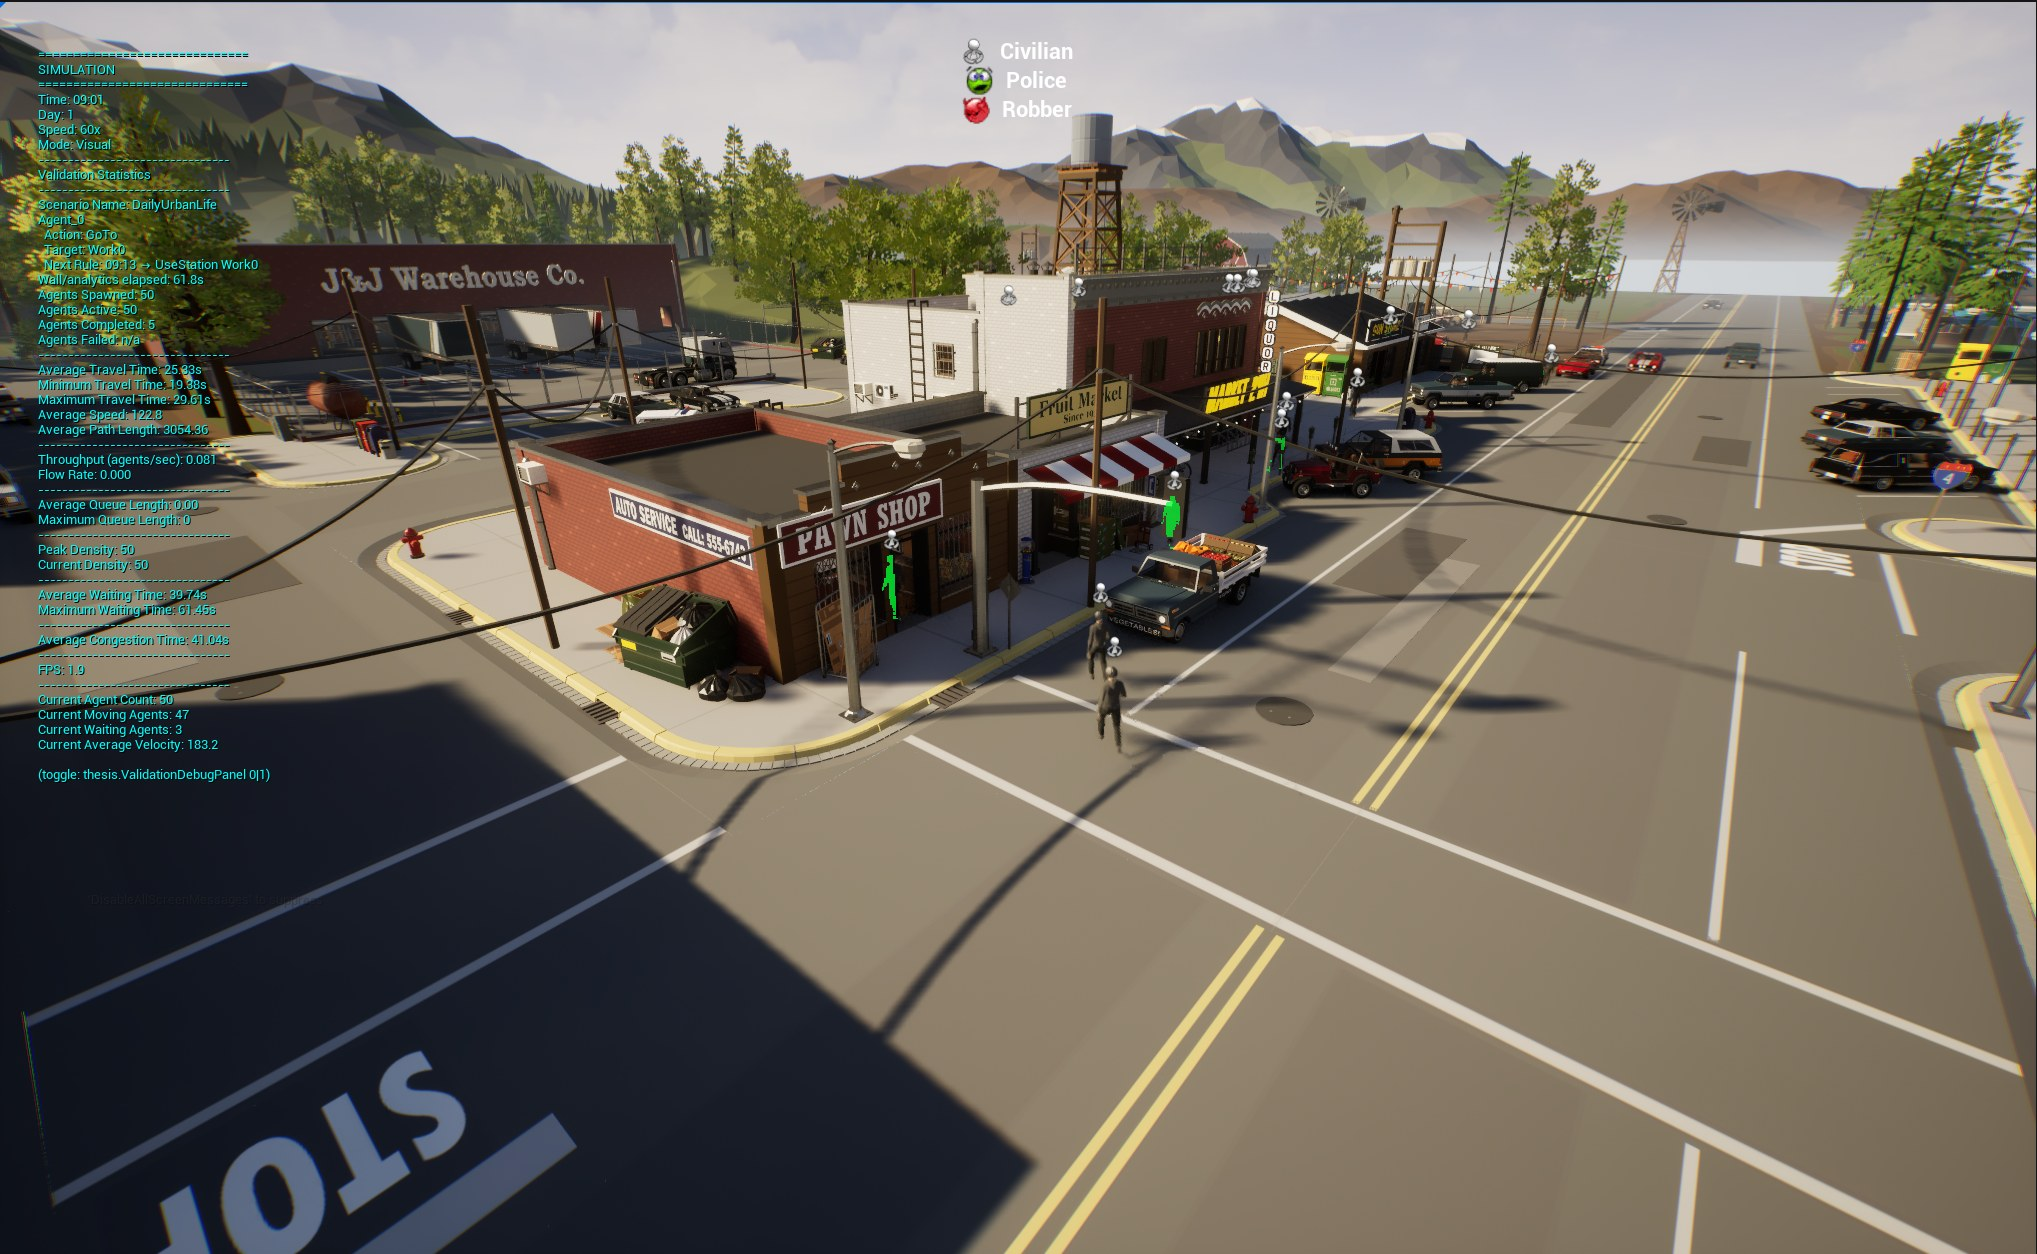
\includegraphics[width=0.85\textwidth]{images/shots/dul_overview.jpg}
\caption[Daily Urban Life map during the morning]{Daily Urban Life map during the morning in Visual mode, where each figure is a person following their own schedule and the validation panel is on the left.}
\label{fig:app-dul-overview}
\end{figure}

\begin{table}[H]
\centering
\small
\begin{tabular}{|l|c|}
\hline
\rowcolor{headgray}\textbf{Outcome} & \textbf{\shortstack{Percent of the authored\\rules, walks or visits}} \\
\hline
\tabinput{analysis/tables/dul_rows.tex}
\end{tabular}
\caption[Daily Urban Life outcomes]{Daily Urban Life outcomes with 50 people as a share of the authored rules, of the walks or of the station visits (mean of five runs).}
\label{tab:app-dul}
\end{table}

The schedule leaves enough time for walking, as \texttt{Agent\_0} has 18 simulated minutes between leaving for \texttt{Work0} and sitting at their desk, and the walk is about 150~m long. Two things delay rules: competition at shared places and long walks to crowded target points. Two shifts share 25 desks, and of the 481 desk requests in the five runs, 260 queued and 300 ended in a completed work session, and these counts overlap because a request that queued can still end in a completed session. The wait per station visit averaged 1.7 simulated minutes, and queueing was 34\% of the start delay of station rules (\cref{fig:app-start-delay}). A desk queue can outlast the time until the person's break, and since the break releases the place as designed, 7 to 32 reserved stations per run were left before the person reached them. The scenario therefore measures competition for work sessions, which the time scale of Visual mode had hidden, because there a walk took longer than the schedule allowed for it.

Single-point targets still take time (\cref{fig:app-dul-arrivals}), as 75\% of the walks to \texttt{Work3} arrived, against 90 to 100\% at the other work areas. The median walk to a work area took 1.6 simulated minutes, close to the 1.3 minutes that 150~m at 2~m/s needs, but the walks to these shared single points have a long tail. Of the 235 walks that arrived, 43 took more than 5 minutes while the person milled about a crowded point, and 7 of them, like all 15 walks that failed, lasted until the GoTo time-out. A person who keeps being pushed around near a crowded point without coming to rest, or who rests just outside the arrival radius, ends their walk only at that time-out. The walk then counts as arrived if the person is within 180~cm and as failed otherwise, and the time-out lasts 180 real seconds, which Accurate mode does not convert and which the clock counts as 90 simulated minutes. These long walks raise the mean walk to a work area to 7.5 simulated minutes, and these walks account for 95\% of the late minutes. Without the 7 walks that ended on the time-out, the mean is 5.0 minutes, so the time-out adds about a third to the mean, while crowding at the single points causes the rest of the tail. A few people never left home, because no sidewalk path started where they stood, and overall, 94\% of walks counted as arrived, an upper bound by the definition of \cref{sub:app-recording}.

\begin{figure}[H]
\centering
\begin{tikzpicture}
\begin{axis}[
  width=0.95\textwidth, height=5.6cm,
  ybar=3pt, bar width=14pt, ymin=0, ymax=112,
  ytick={0,25,50,75,100},
  symbolic x coords={Work0,Work1,Work2,Work3,Work4,Work5,Work6}, xtick=data,
  ylabel={Walks that arrived (\%)}, xlabel={Work area},
  % axis lines resets the enlargement, so enlarge x limits must follow it
  axis lines=left, enlarge x limits=0.08, ymajorgrids, grid style={black!12},
  tick label style={font=\small}, label style={font=\small},
  /pgf/number format/assume math mode=true,
  nodes near coords, every node near coord/.append style={font=\footnotesize, inner sep=1.5pt}]
\addplot[fill=cBlue, draw=cBlue!70!black] table[x=area, y=accurate] {analysis/data/dul_work_arrivals.dat};
\end{axis}
\end{tikzpicture}
\caption[Walks that arrived at each work area]{Share of walks that arrived at each work area (five runs).}
\label{fig:app-dul-arrivals}
\end{figure}

\section{Shopping Center: Mall A and Mall B}
\label{sec:app-mall}

\label{sub:app-mall-authored}

Each shopping center has its own schedule for ten people: 53 rules in Mall A, of which 28 are \texttt{MoveTo}, 15 \texttt{UseStation} and 10 \texttt{Idle}, and 59 in Mall B, which adds four walks, one station use and the single \texttt{Interact}. Every person waits at an entrance, browses one or two shops, uses a shop desk or a seat, eats, and leaves. In Mall A, nine people eat, and the meal is a two-stage pipeline: a food counter for 10 minutes, then a food table for 14 (\cref{lst:malla-pipeline} in \cref{chap:contribution}). The table is chosen only when the counter stage ends, so a slow counter delays the table request. \Cref{fig:app-malla} shows the entrance of Mall A and its levels, as the map has more than one floor.

\begin{figure}[H]
\centering
\begin{subfigure}[b]{0.32\textwidth}\centering
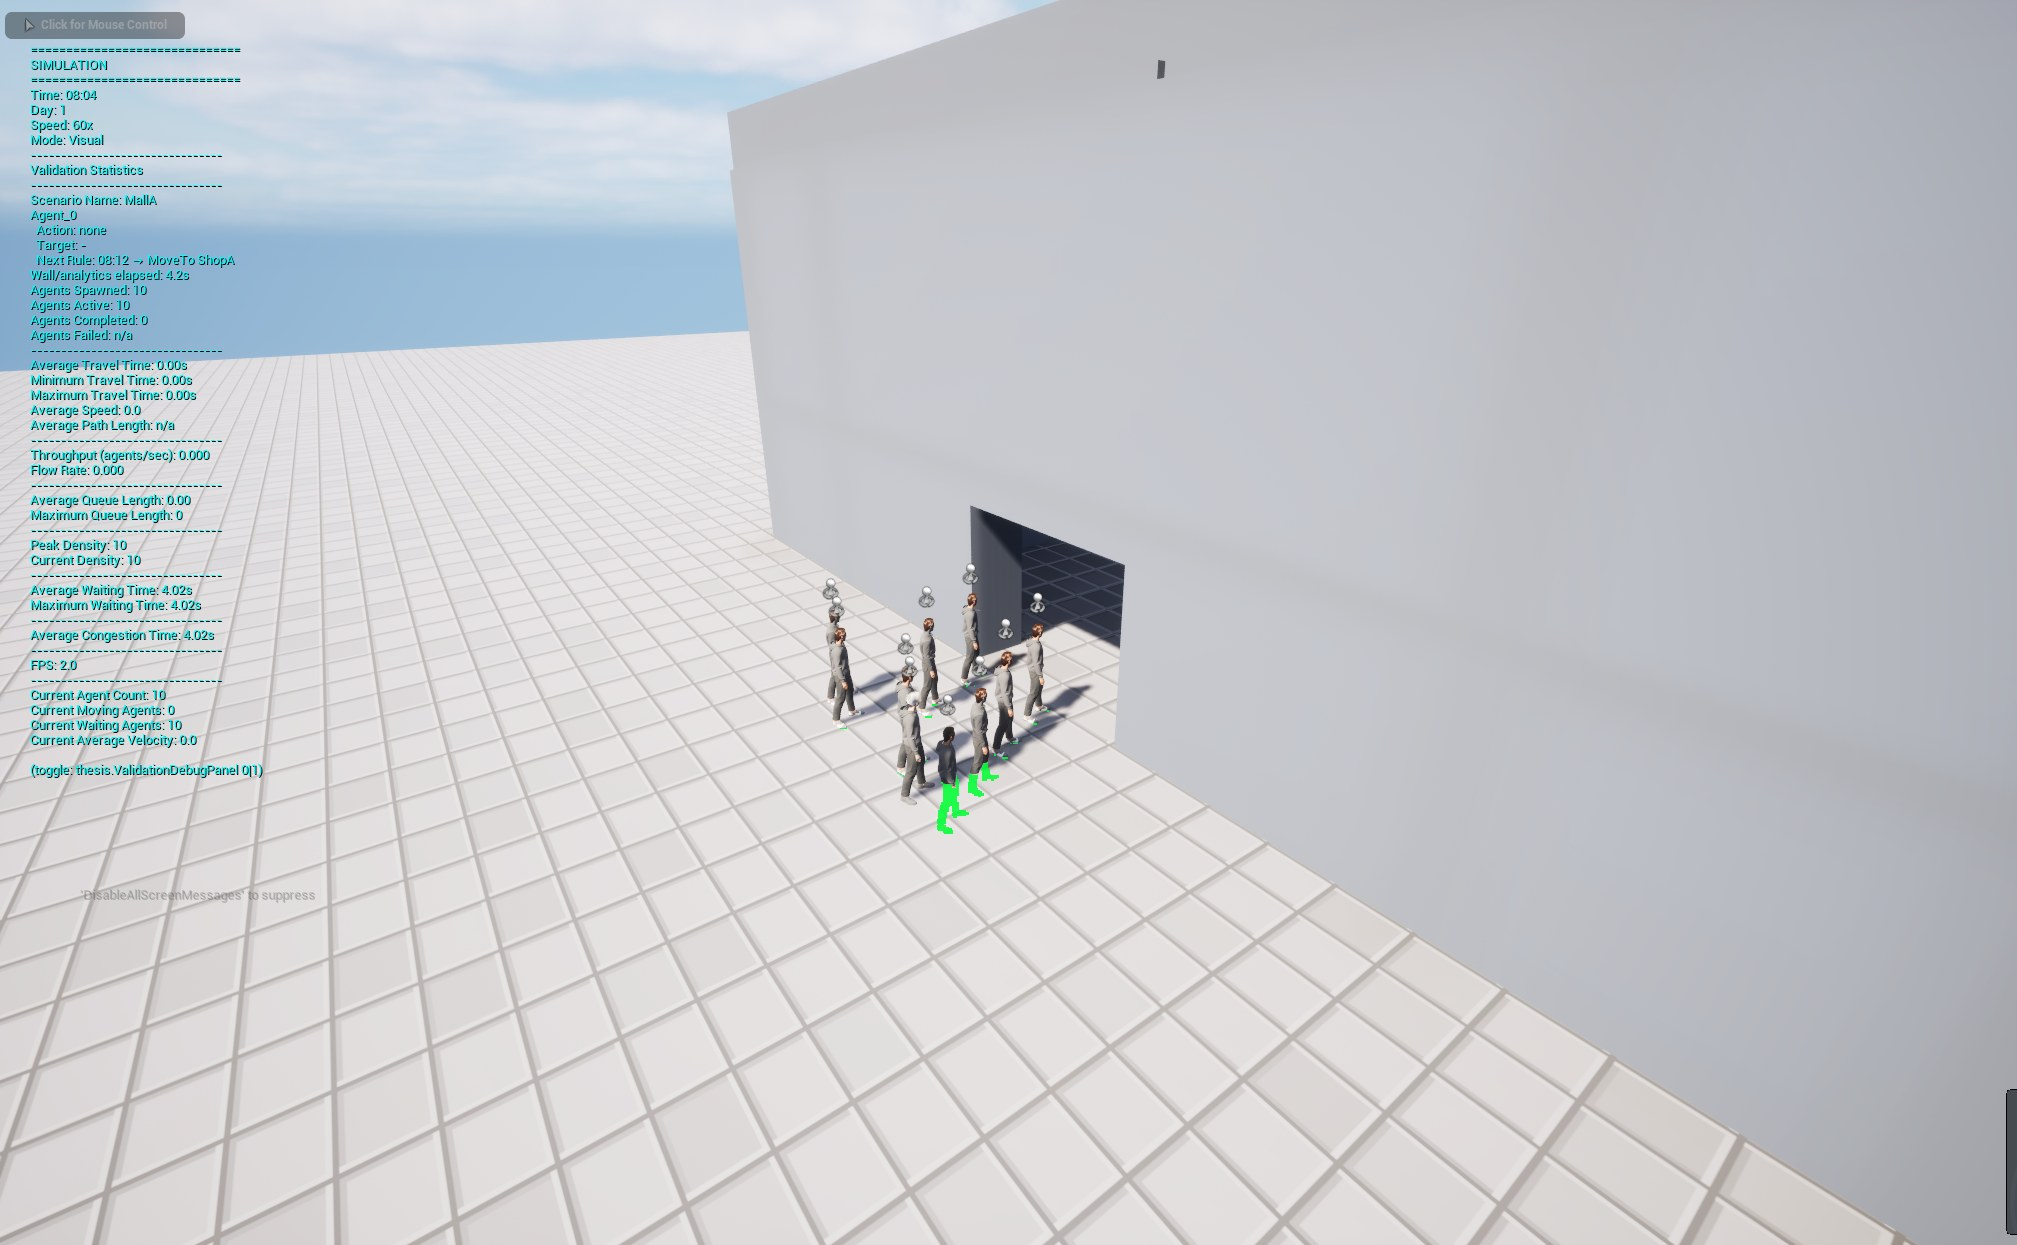
\includegraphics[width=\linewidth]{images/shots/malla_entrance.jpg}
\caption{The entrance}
\end{subfigure}\hfill
\begin{subfigure}[b]{0.32\textwidth}\centering
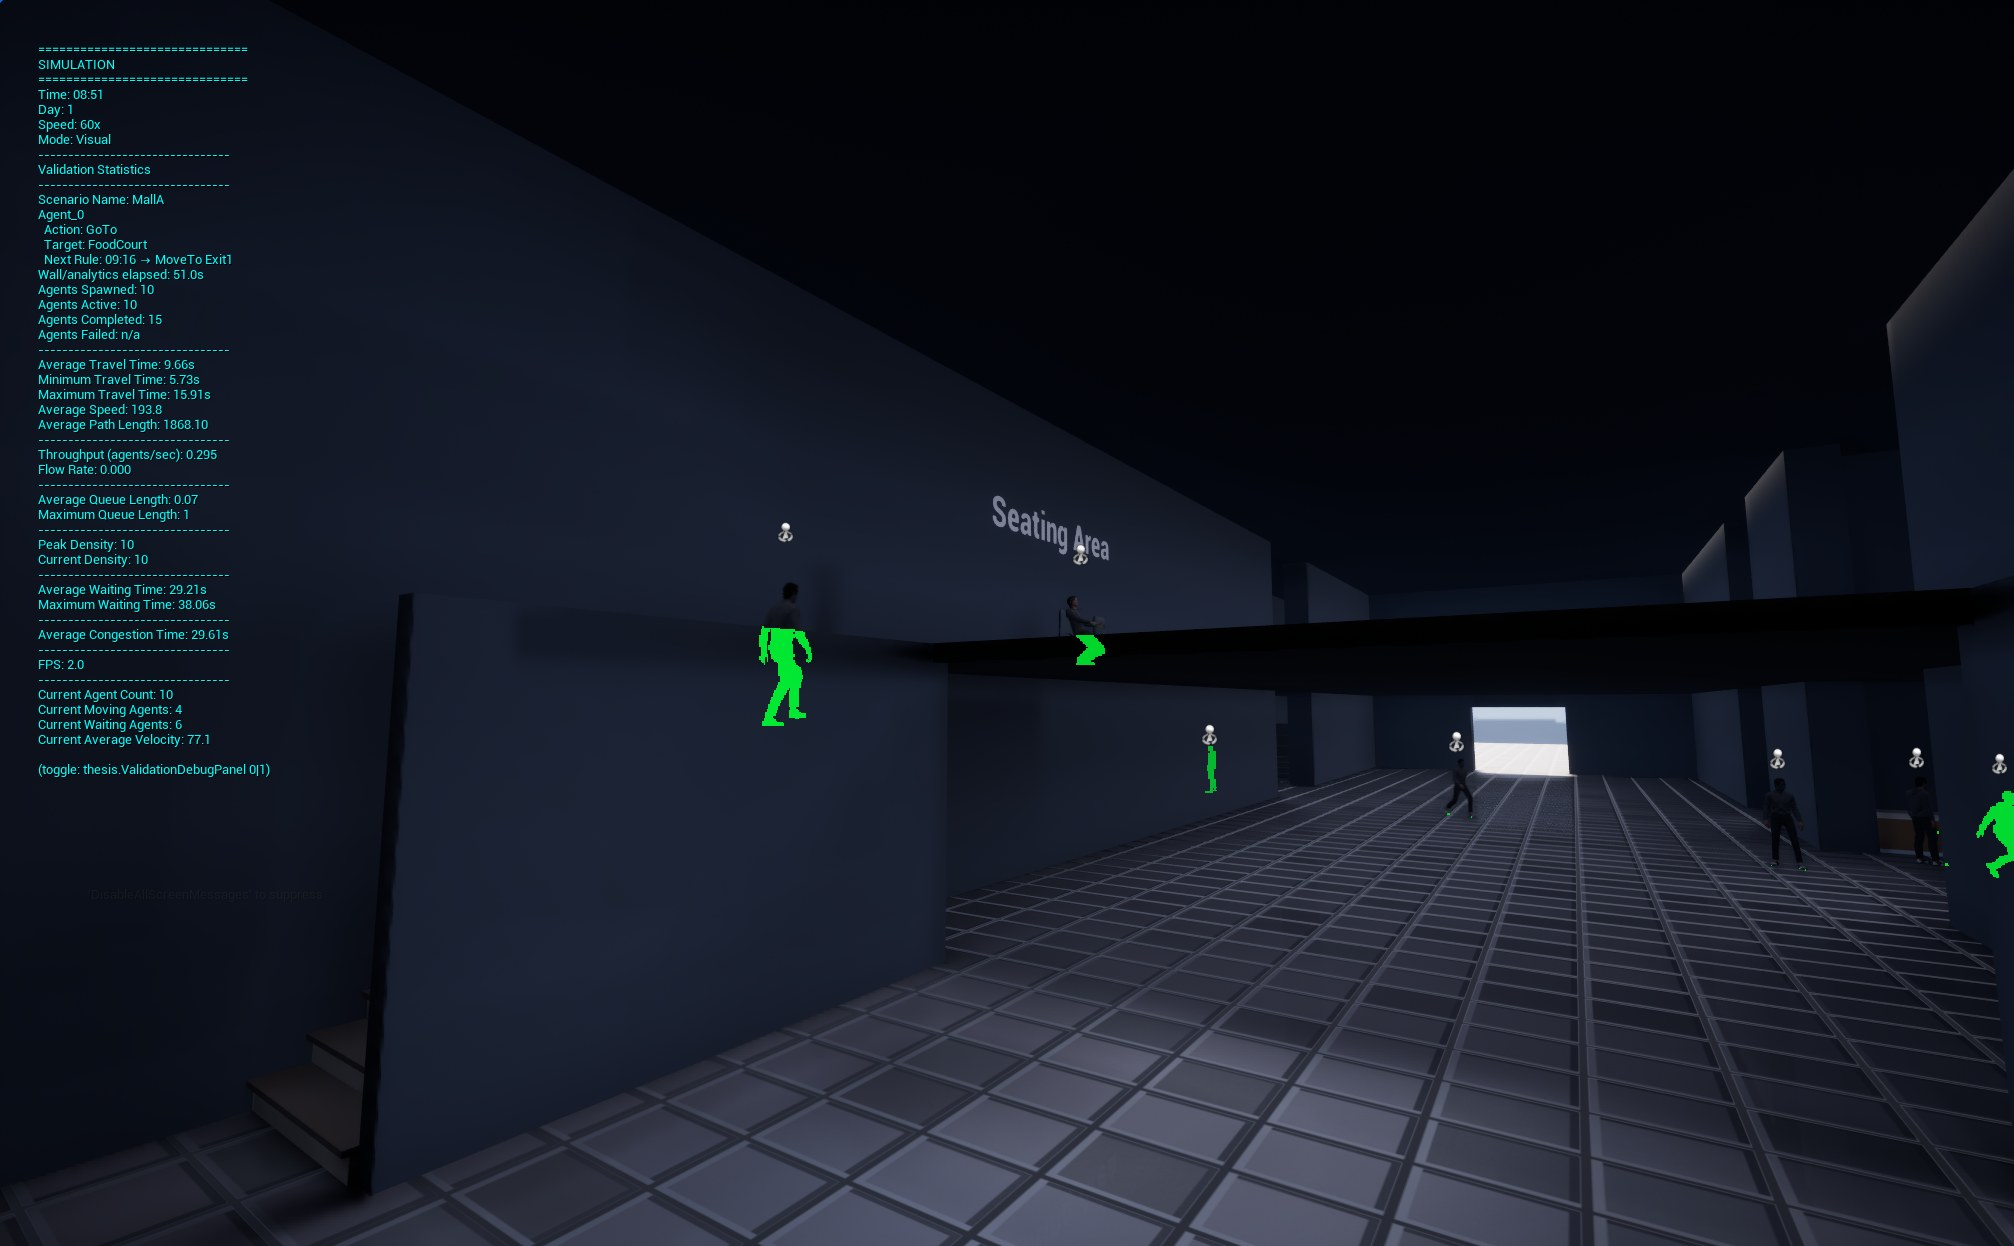
\includegraphics[width=\linewidth]{images/shots/malla_upper_level.jpg}
\caption{Its levels}
\end{subfigure}\hfill
\begin{subfigure}[b]{0.32\textwidth}\centering
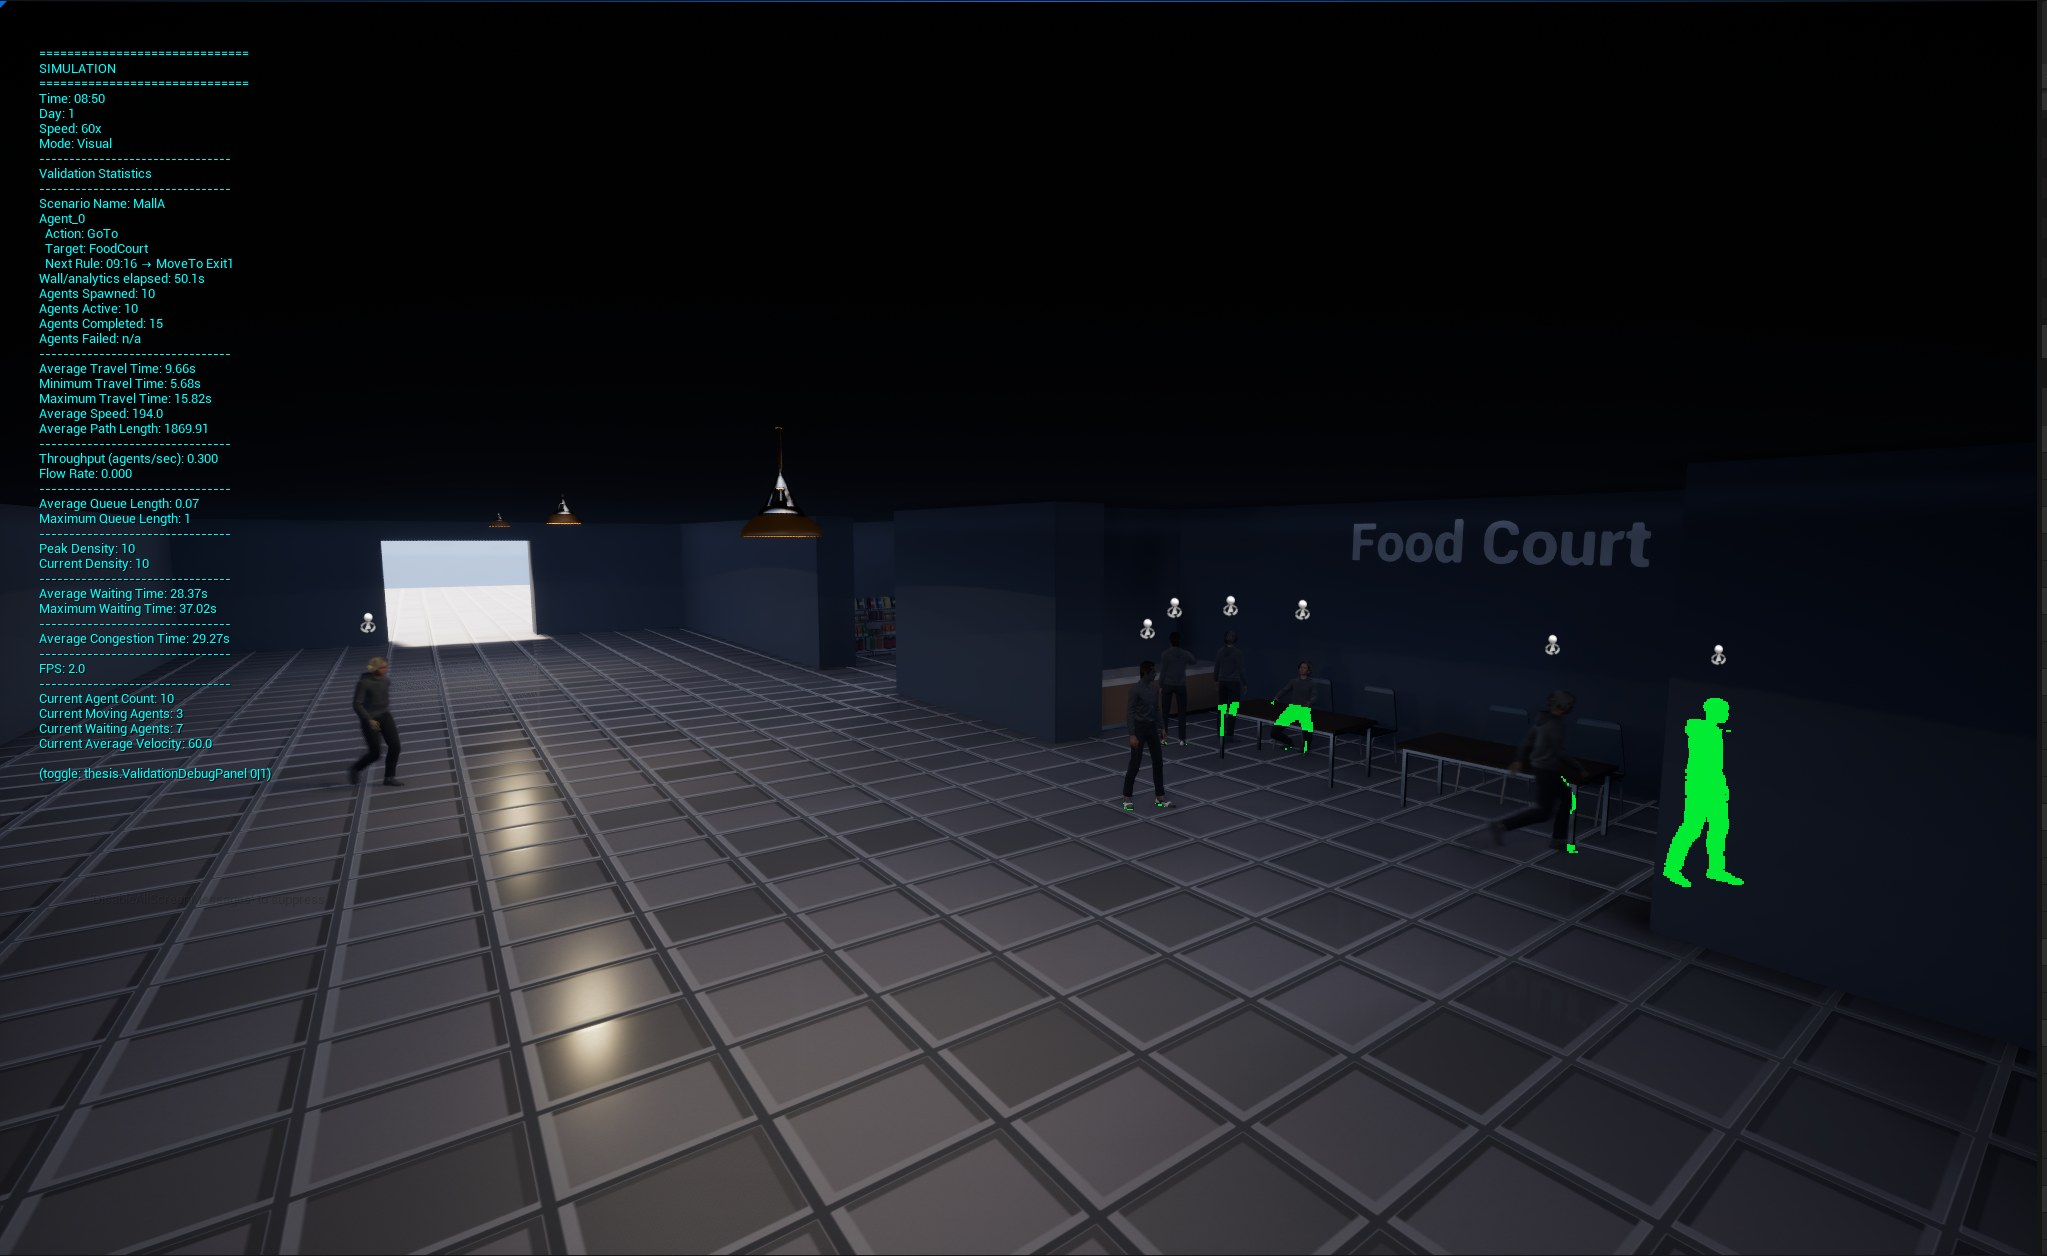
\includegraphics[width=\linewidth]{images/shots/malla_foodcourt.jpg}
\caption{The food court}\label{fig:app-malla-food}
\end{subfigure}
\caption[Mall A]{Mall A, with (a) its entrance, (b) a view of its levels and (c) its food court, where a meal uses a counter and then a table.}
\label{fig:app-malla}
\end{figure}

Mall B keeps the same ten people and their schedules with three changes: four people eat at a second food court, service points have two places instead of one, and \texttt{Agent\_0} first walks to a button (\texttt{MoveTo} at 08:04) and presses it (\texttt{Interact} at 08:08). The button opens a second entrance, where the odd-numbered people start (\cref{fig:app-mallb}).

\begin{figure}[H]
\centering
\begin{subfigure}[b]{0.32\textwidth}\centering
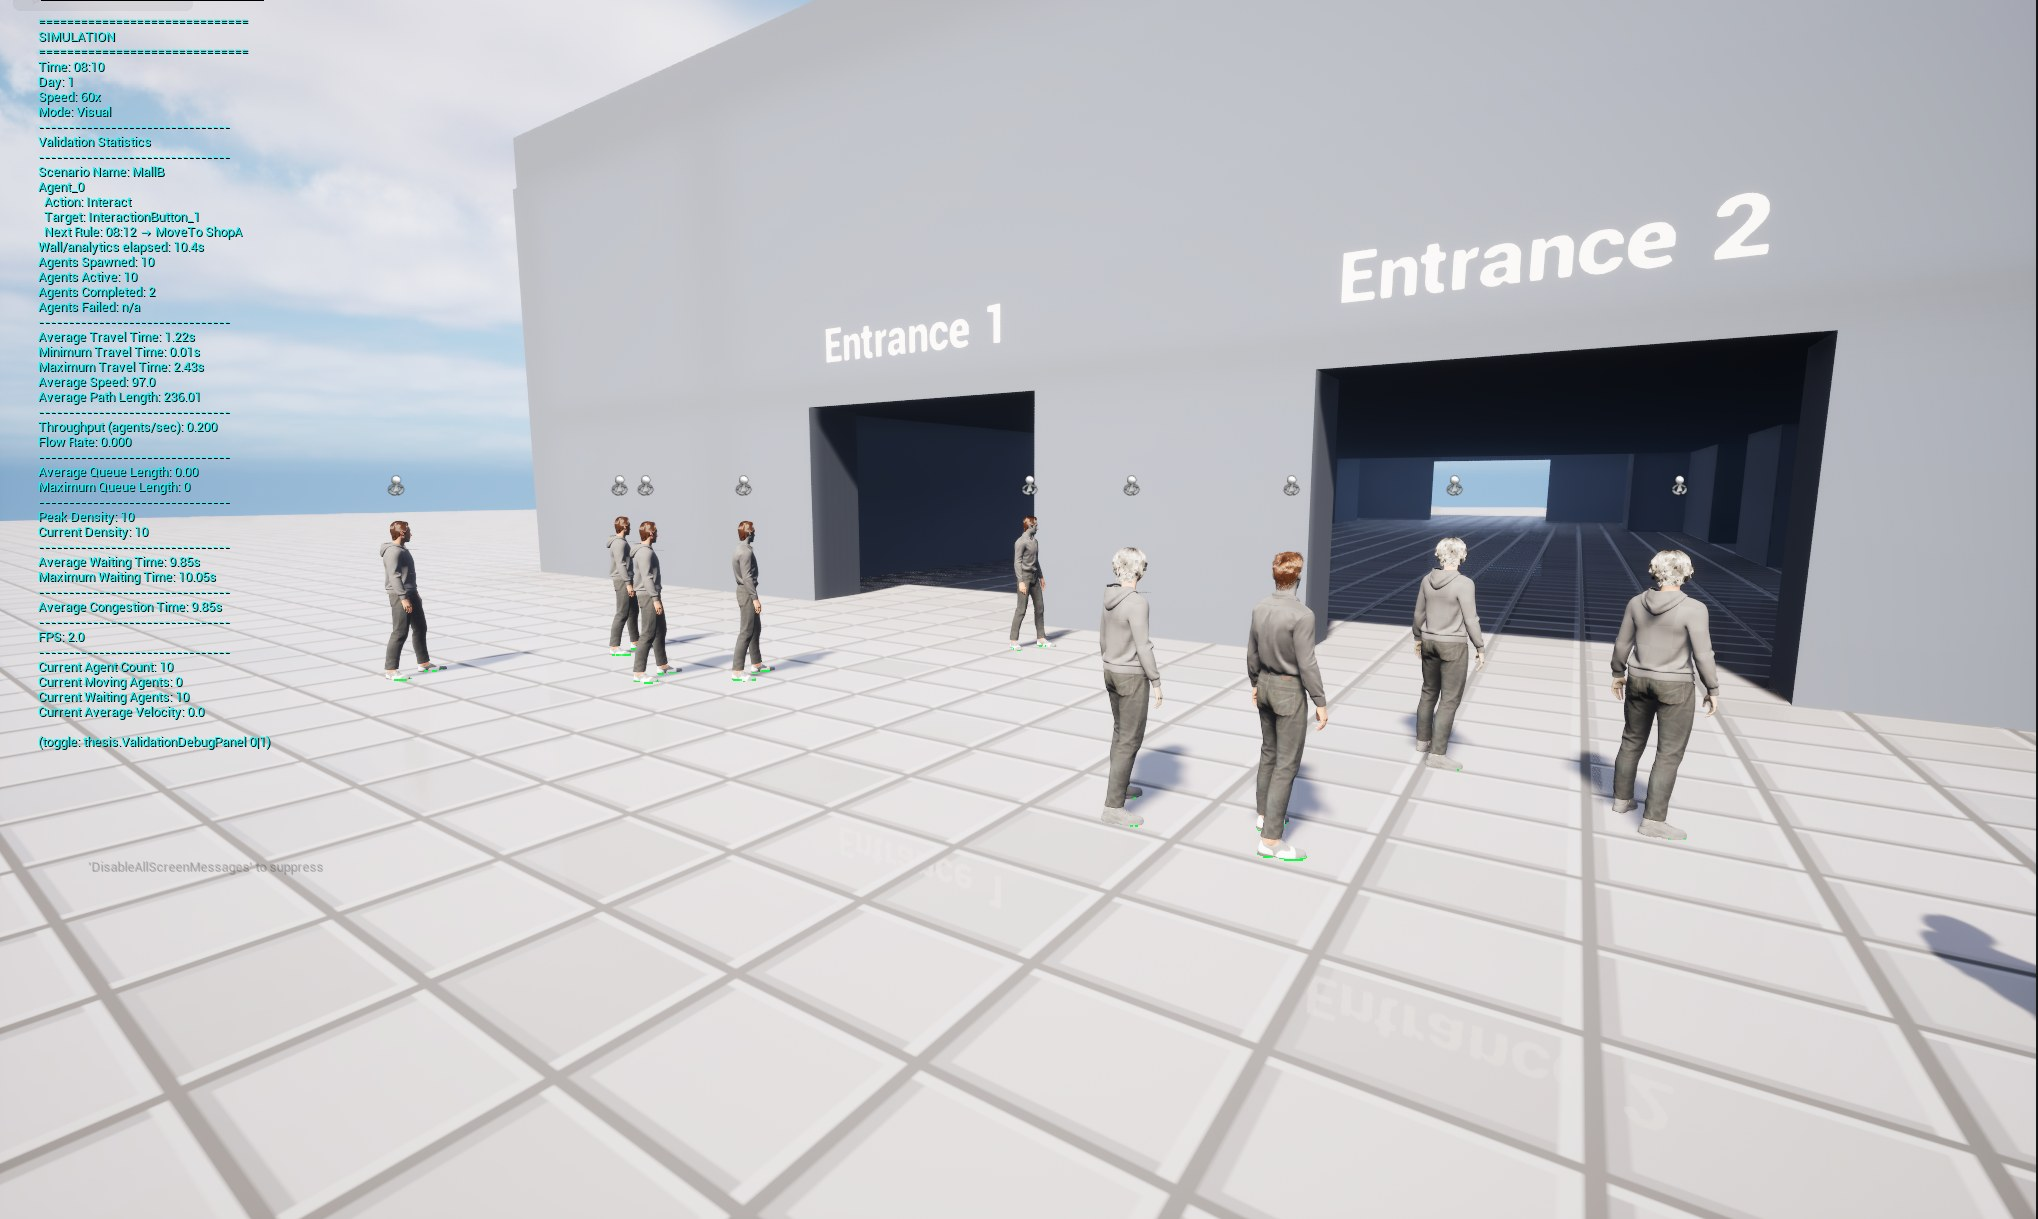
\includegraphics[width=\linewidth]{images/shots/mallb_entrances.jpg}
\caption{The two entrances}
\end{subfigure}\hfill
\begin{subfigure}[b]{0.32\textwidth}\centering
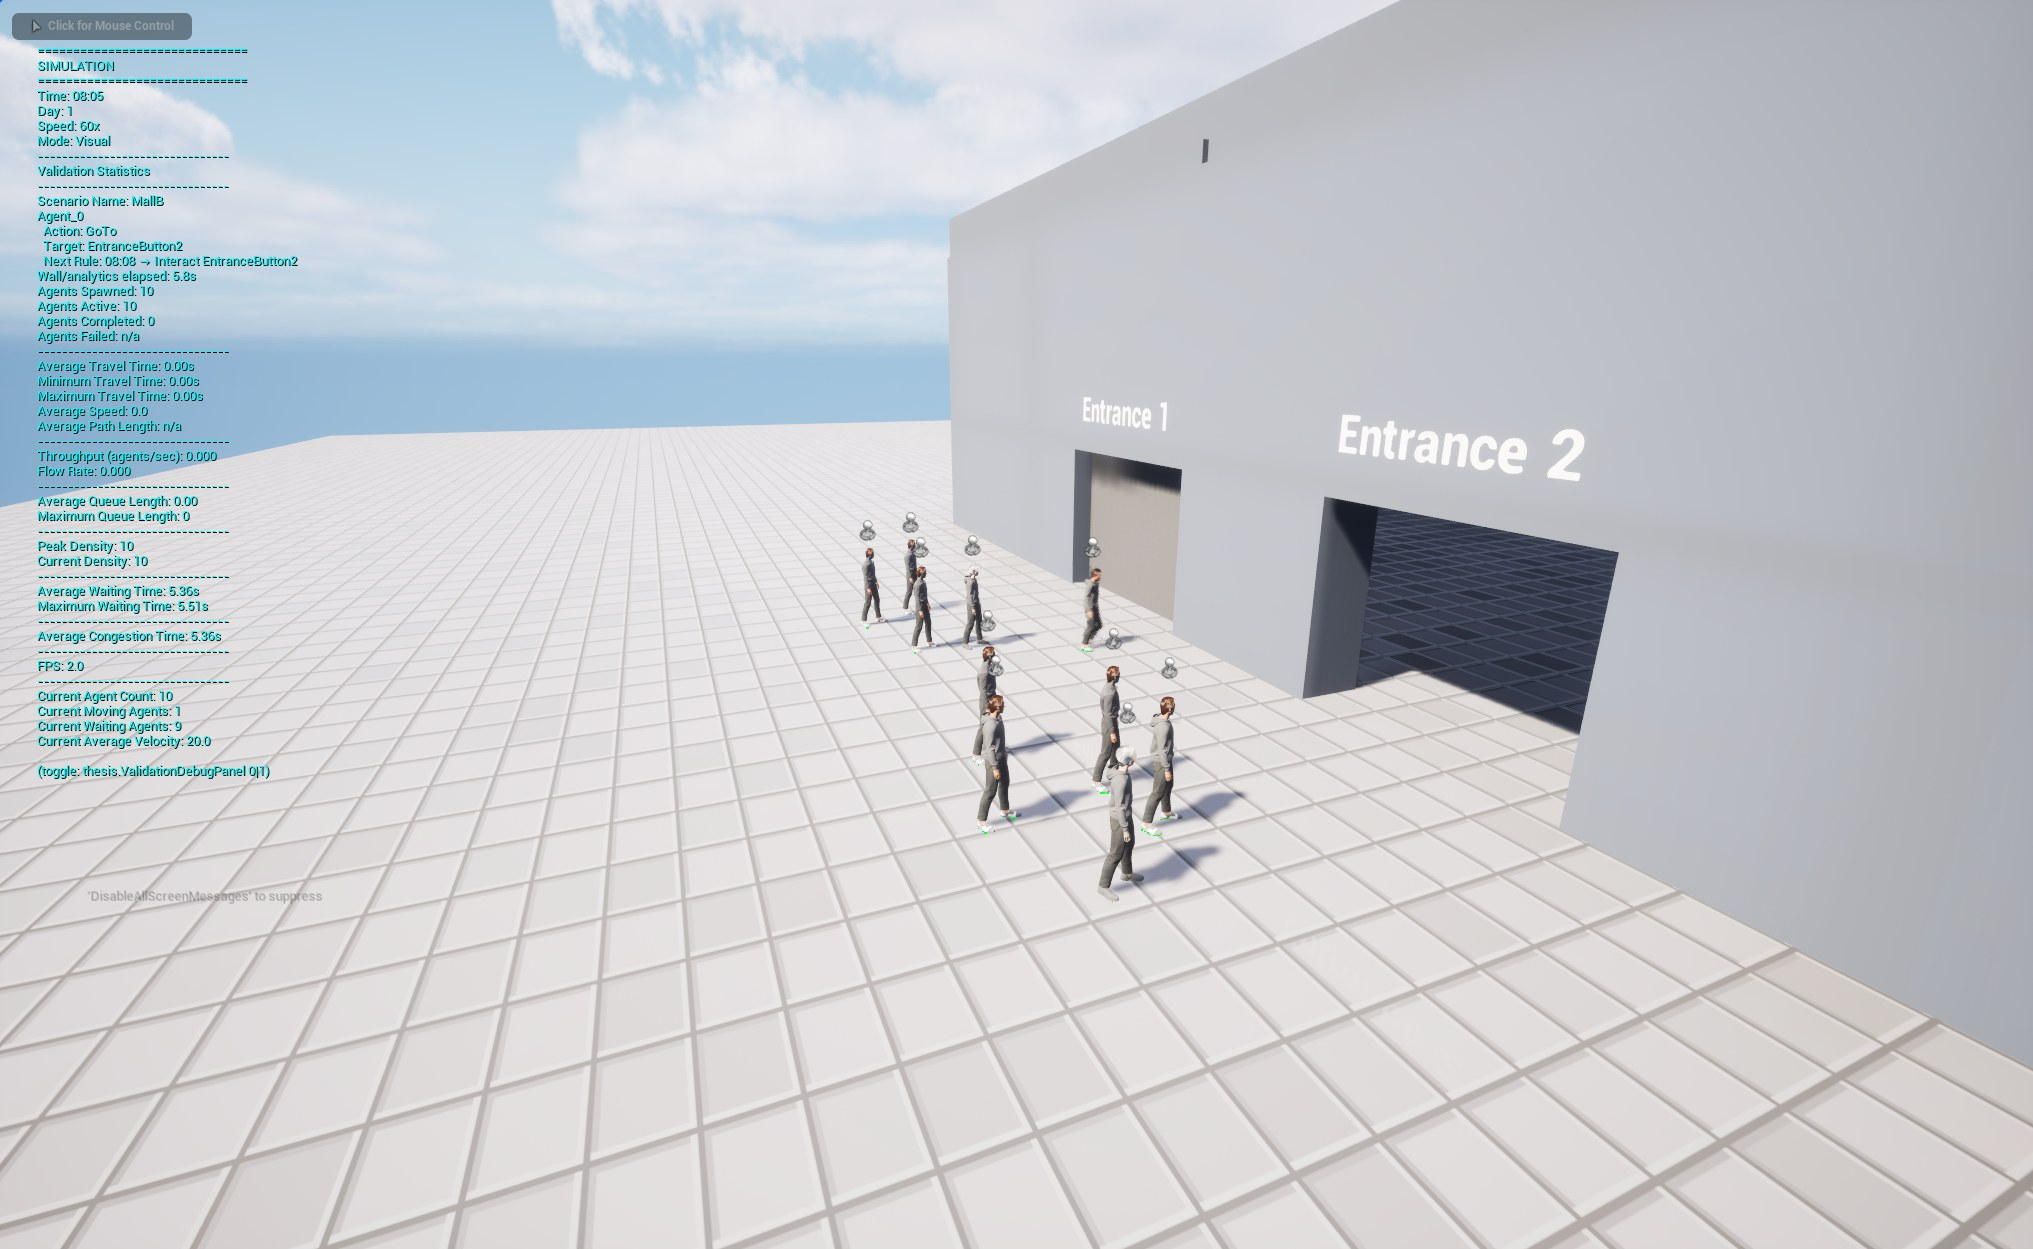
\includegraphics[width=\linewidth]{images/shots/mallb_interact.jpg}
\caption{Walking to the button}
\end{subfigure}\hfill
\begin{subfigure}[b]{0.32\textwidth}\centering
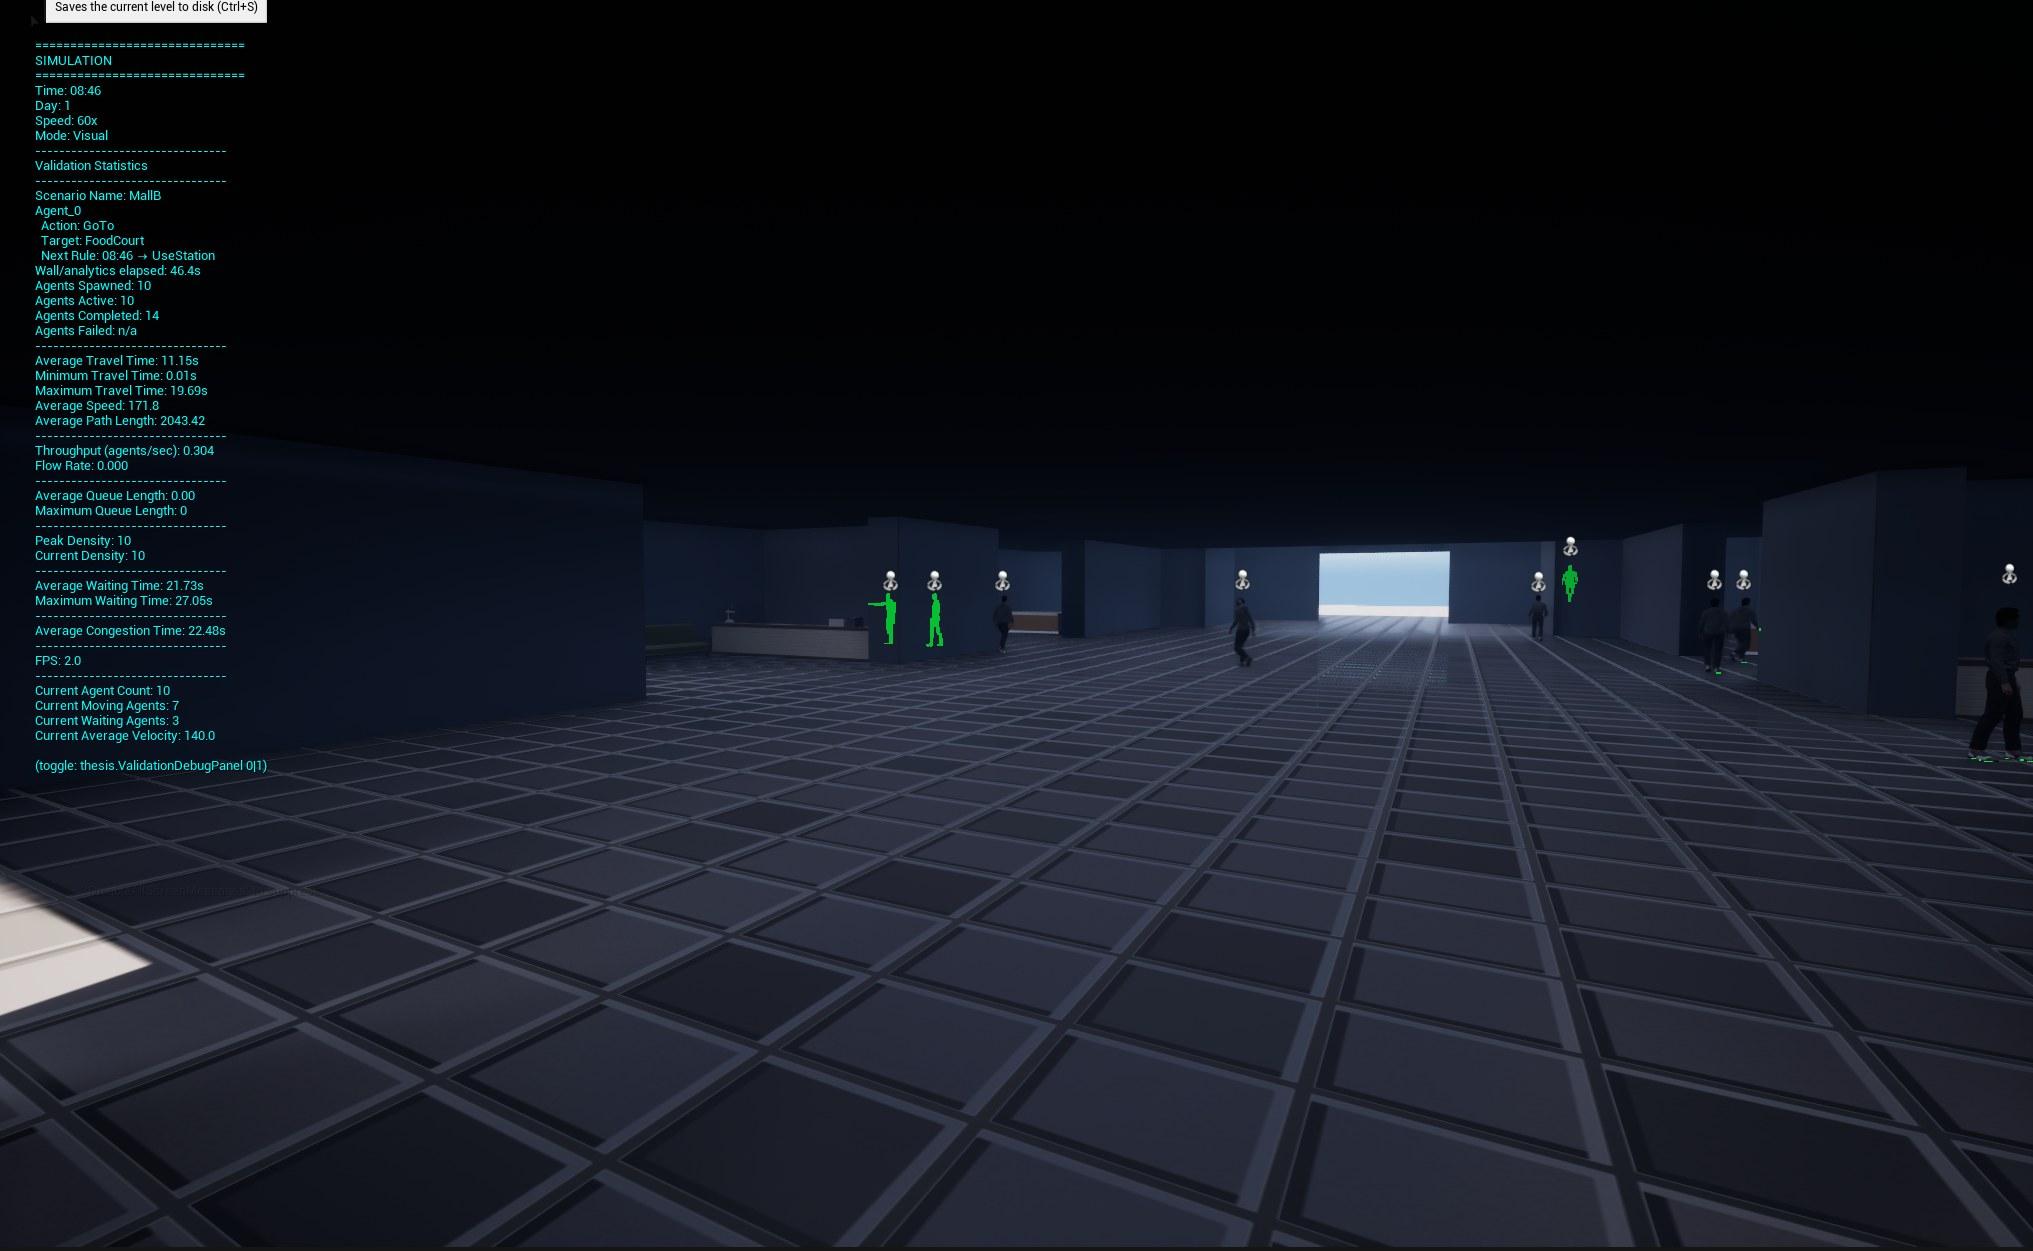
\includegraphics[width=\linewidth]{images/shots/mallb_interior.jpg}
\caption{The interior}
\end{subfigure}
\caption[Mall B]{Mall B, with (a) its two entrances, (b) a person walking to the button that opens the closed entrance with the \texttt{Interact} action, and (c) its interior.}
\label{fig:app-mallb}
\end{figure}

Both maps have two shops with desks, a seating area, and a food court built as a super station with four counters and four tables (\cref{fig:app-malla-food}). Mall B adds \texttt{FoodCourt2}, the button, and a gate that removes its area from the navigation mesh while closed. The infrastructure manager places people at the entrances and sets the capacity of every station whose actor tag or identifier matches a configured name, so that the capacity tests can change one kind of station at a time. A place is reserved when the rule fires, and a person who finds every station of the requested type full joins the queue of the first one and waits where they stand. The walk to the food court took 0.4 simulated minutes on average in Mall A, well within the 10 minutes that \texttt{Agent\_0}'s schedule allows.

\subsection{Capacity experiments}
\label{sub:app-mall-capacity}

We kept the Mall A map and schedule fixed and changed one kind of station at a time (shop desks, counters or tables) to one, two or three places, with five runs per setting, later extended to 30 runs per setting (\cref{fig:app-capacity}). In the counter and table tests, the shop desks kept their editor capacity, which allowed two people at one desk, so the one-place bars of the three groups are not the same configuration, although their medians coincide.

\begin{figure}[H]
\centering
\begin{tikzpicture}
\begin{axis}[
  width=0.9\textwidth, height=5.8cm,
  ybar=3pt, bar width=18pt, ymin=0, ymax=1.65,
  ytick={0,0.5,1,1.5},
  symbolic x coords={1,2,3}, xtick=data, xticklabels={One place, Two places, Three places},
  ylabel={Median wait per visit (min)},
  axis lines=left, ymajorgrids, grid style={black!12},
  tick label style={font=\small}, label style={font=\small},
  /pgf/number format/assume math mode=true,
  enlarge x limits=0.22, legend image code/.code={\draw[#1] (0cm,-0.08cm) rectangle (0.3cm,0.14cm);},
  legend style={draw=none, fill=none, at={(0.5,1.02)}, anchor=south, legend columns=3, font=\small, /tikz/every even column/.append style={column sep=10pt}},
  nodes near coords, every node near coord/.append style={font=\scriptsize, inner sep=1.5pt, /pgf/number format/fixed, /pgf/number format/precision=2}]
\addplot[fill=cSky, draw=cSky!60!black] table[x=places, y=desks] {analysis/data/capacity30_median.dat};
\addlegendentry{Shop desks changed}
\addplot[fill=cOrange, draw=cOrange!60!black] table[x=places, y=counters] {analysis/data/capacity30_median.dat};
\addlegendentry{Food counters changed}
\addplot[fill=cGreen, draw=cGreen!60!black] table[x=places, y=tables] {analysis/data/capacity30_median.dat};
\addlegendentry{Food tables changed}
\end{axis}
\end{tikzpicture}
\caption[Median wait per visit by number of places]{Median wait per station visit in Mall A by number of places (simulated minutes, 30 runs per setting, lower is better), with the full statistics in \cref{tab:app-capacity}.}
\label{fig:app-capacity}
\end{figure}

The one-place baseline differs between the two rounds, at 0.81 simulated minutes over the five seeds and 0.84 over the 30 runs, so each value below is quoted with the round it comes from. In the first five runs per setting, two or three places at the tables lowered the wait per visit from 0.81 to 0.51 simulated minutes in all five runs ($p=0.008$). More places at the counters raised it to 1.21 with two places ($p=0.008$) and 1.35 with three ($p=0.10$), and the queue joins explain why. With one place per counter, 10 counter requests and 5 table requests queued over the five runs. With two or three counter places, the counter queues disappeared, but more diners reached the tables at the same time, and as the tables kept one place each, 10 and 11 table requests queued, so the bottleneck moved down the pipeline and the wait grew. With one table place, only 5 of 45 table requests queued in five runs, about one queued visit per run, so the lower wait with more table places is the removal of that visit. No person ever joined a desk queue, and the desk settings made no difference ($p=1.0$). Over 30 runs per setting (\cref{fig:app-capacity,tab:app-capacity}), the medians show the same pattern: 0.84 minutes with one place, 1.34 and 1.26 with two and three counter places ($p<0.001$), 0.51 with two or three table places ($p<0.001$) and 0.84 for every desk setting ($p=0.89$). The table result is a difference of about 20 seconds per visit, small against a 24-minute meal, so what matters is its direction, which behaves as a tandem queue should and which the lunch rush below repeats with waits of several minutes. The mean with three counter places (2.43 minutes) is not a valid summary, because in 3 of its 30 runs a diner was admitted to a table they never reached and held it until the run ended, with one or two people queued behind them. These runs averaged 7.5 to 16.0 minutes of wait per visit, while the other 27 runs averaged 1.25 minutes (\cref{sub:app-edge-cases}).

The logs also explain why queues persist while equivalent stations are free. All queue joins of a given kind went to a single station, because a queued person stays with the first matching station even when an equivalent one frees up. The capacity comparisons therefore hold under this selection policy, and one shared queue per area could change their sizes. A place is also held while its owner walks to it, though briefly at the real walking pace: in Mall A, a person reserved a counter on average 0.3 minutes and a seat 0.6 minutes before reaching it.

\subsection{A lunch rush}
\label{sub:app-mall-rush}

Ten people seldom compete, so we also ran a lunch-rush variant of the Mall A schedule, with ten runs per setting (\cref{tab:app-rush}). In this variant, the schedule sends all nine diners to the food court at 08:40 and has them request a counter at 08:50, they leave no earlier than 09:20, and the other rules are unchanged. We did not add people by copying them, because with 50 copies of the authored schedule the shared single-point targets jammed. In five such runs, only 26 to 77 of 87 to 107 walks arrived, 148 to 200 of the 265 rules were dispatched and 11 to 41 station services were completed.

\begin{table}[H]
\centering
\footnotesize\setlength{\tabcolsep}{3pt}
\begin{tabular}{|l|c|c|c|c|c|c|c|c|}
\hline
\rowcolor{headgray}\textbf{Stations changed} & \textbf{Places} & \textbf{\shortstack{Median\\wait}} & \textbf{\shortstack{Range\\over runs}} & \textbf{\shortstack{Mean wait\\(SD)}} & \textbf{\shortstack{Queued visits\\per run}} & \textbf{\shortstack{Start\\delay}} & \textbf{\shortstack{Start delay spent\\queueing (\%)}} & \textbf{$p$} \\
\hline
\tabinput{analysis/tables/rush_rows.tex}
\end{tabular}
\caption[Mall A during a lunch rush]{Wait per station visit and start delay in Mall A during a lunch rush with ten runs per setting, in simulated minutes, where SD is the standard deviation and $p$ compares three places with one, and where the start delay covers the counter stage only, so a queue that moved to the tables appears in the wait per visit and not in that column.}
\label{tab:app-rush}
\end{table}

In every rush run, one of the nine diners could not get within the arrival radius of the crowded food-court point, and their walk timed out before it reached the counter stage, so a run records eight counter requests rather than nine and each setting 80 over its ten runs. With one place per counter, 39 of the 80 counter requests queued, the wait per visit averaged 4.6 simulated minutes (median 4.8), and queueing was 92\% of the start delay of station rules. Three places per counter removed the counter queues but moved them to the tables, which kept one place: 40 of 80 table requests queued, later pipeline stages queued for 14.9 minutes on average, and the wait per visit rose to 8.6 minutes (median 5.9, $p<0.001$). Three places per table lowered the wait only slightly (4.4 minutes, median 4.6, $p=0.002$), because the counters, which kept their editor capacity in the table tests, stayed the bottleneck, with 39 of 80 counter requests queued and none at the tables. Under contention, extra places at one stage of the pipeline moved the queue to the next stage that was short of capacity.

\subsection{Where late minutes come from}
\label{sub:app-mall-late}

Late starts were rare, as between 0\% and 4\% of the dispatched rules started late in the capacity settings, and the few late minutes in Mall A were mostly spent finishing a previous activity rather than walking. Lateness stops at dispatch, however, so \cref{fig:app-start-delay} also splits the whole start delay of station rules. In Mall A, a station rule started its service on average 1.0 simulated minute after it became eligible, with no lateness, 0.7 minutes queueing for a place and 0.3 minutes walking to the reserved station. Queueing was 67\% of the start delay over all 50 Mall A runs and 76\% in Mall A as authored, and later pipeline stages, such as the table after the counter, queued for 1.2 minutes on average. The start delay covers only the first stage of a pipeline, so with two or three counter places it shows no queueing, while the table stage queued for 3.2 to 3.6 minutes on average. The 105 Daily Urban Life station rules that never started are also left out of its mean, and in Mall B, where no person queued, the start delay was the walk alone. With walking at its real pace, waiting for shared stations is the largest part of the gap between authored and realized times in the shopping centers, while in Daily Urban Life long walks to crowded target points take a larger share (\cref{sub:app-dul-results}).

\begin{figure}[H]
\centering
\begin{tikzpicture}
\begin{axis}[
  width=0.9\textwidth, height=5cm,
  xbar stacked, bar width=14pt, xmin=0, xmax=6,
  ytick={0,1,2}, yticklabels={Mall A, Mall B, Daily Urban Life}, y dir=reverse,
  xlabel={Mean start delay of a station rule (min)},
  axis lines=left, xmajorgrids, grid style={black!12},
  tick label style={font=\small}, label style={font=\small},
  /pgf/number format/assume math mode=true,
  enlarge y limits=0.35, legend image code/.code={\draw[#1] (0cm,-0.08cm) rectangle (0.3cm,0.14cm);},
  legend style={draw=none, fill=none, at={(0.5,1.03)}, anchor=south, legend columns=4, font=\small, /tikz/every even column/.append style={column sep=8pt}}]
\addplot[fill=cPurple, draw=cPurple!60!black] table[y=y, x=lateness] {analysis/data/start_delay_split.dat};
\addlegendentry{Lateness $\ell$}
\addplot[fill=cVerm, draw=cVerm!60!black] table[y=y, x=queue] {analysis/data/start_delay_split.dat};
\addlegendentry{Queueing $q$}
\addplot[fill=cBlue, draw=cBlue!60!black] table[y=y, x=walk] {analysis/data/start_delay_split.dat};
\addlegendentry{Walking $w$}
\addplot[fill=cOrange, draw=cOrange!60!black] table[y=y, x=position] {analysis/data/start_delay_split.dat};
\addlegendentry{Positioning $p$}
\end{axis}
\end{tikzpicture}
\caption[Start delay of station rules]{Start delay of station rules split into its parts (simulated minutes), with the values in \cref{tab:app-start-delay}.}
\label{fig:app-start-delay}
\end{figure}

\subsection{Mall A against Mall B}
\label{sub:app-mall-layouts}

In Mall B, no person ever queued, and its rules started on time about as often as in Mall A, but because schedule, layout and capacities all differ, the comparison does not isolate the effect of layout. In Visual mode, these runs had exposed an edge case of the reservations, as a reservation has no time-out and a failed path only stops the person, so a person who never reached their reserved station held the place until the run ended. In Accurate mode, no station visit was still open at the end of any layout run, and no walk failed, so this edge case did not affect this comparison. It can still occur, and it dominated three capacity runs with three counter places (\cref{sub:app-mall-capacity}), in which a person admitted to a table never reached it.

\section{Emergency Evacuation}
\label{sec:app-evac}

\label{sub:app-evac-authored}

The evacuation needs one rule (\cref{lst:app-evac}), and the rest is scenario code. The emergency manager starts a fire incident covering the map, raises the alarm for every person and starts a countdown authored as 120 seconds, which keeps its Visual meaning of 120 simulated minutes in Accurate mode. Each person first waits for a reaction delay, authored as 0 to 5 seconds, which Accurate mode turns into 0 to 5 simulated minutes, long for a reaction to an alarm but short against the 120-minute countdown. The person then chooses an exit by a score that combines distance and queue length, asks for a queue place and walks to their slot, and may switch exits every 5 seconds, at most three times.

\begin{lstlisting}[language=XML, caption={The evacuation schedule. The trigger is global and idempotent, so one coordinator is enough.}, label={lst:app-evac}]
<agent id="Agent_0">
  <rule time="08:05"><then action="StartEvacuation"/></rule>
</agent>
\end{lstlisting}

The map is an open floor with walls, two exits, and a safe zone (\cref{fig:app-evac-exits}). Each exit lets one person through every 1.5 real seconds, a constant that Accurate mode does not convert, so an exit serves one person every 45 simulated seconds, far fewer than a real door of that width would pass. The results below therefore test the exit and queue mechanism rather than an evacuation time, and they cannot yet say whether an exit would become a choke point, the question that \cref{chap:intro} opens with. Each exit lays out its queue as slots behind it, at most 25 on this map (the recorded peak at both exits in every run with 100 or 200 people). A person who has passed an exit walks to the safe zone and is counted as safe within 200~cm of its center, and when the countdown ends, every other person becomes a casualty.

\label{sub:app-evac-results}

We ran the evacuation with 50, 100, and 200 people, three times each, made the larger populations by copying the map's people, and repeated every run with a step of 0.25 instead of one simulated second per frame (\cref{fig:app-evac}). At one second per frame, all 50 people passed an exit before the countdown ended, 89 to 100 of 100, and 44 to 75 of 200. At 0.25 seconds per frame, all 50 and all 100 did so in every run, and 57 to 66 of 200.

An exit lets one person through every 45 simulated seconds, so in the 120-minute countdown it could pass 160 people, and two exits 320, but the exits passed at most 51 people each, so their designed capacity does not explain the losses. The losses came from stalled exits: in one run with 100 people and one with 200 at one-second steps, one exit passed at most two people after its queue stalled, and with 200 people both exits passed fewer than 40 at either step. We did not check the positions of the people, but the pattern suggests an edge case of the exit queues. People who cannot get a queue place keep pressing towards the exits, so the person who becomes first in a queue cannot always reach the head slot. Only 10 to 31 people per run were counted as safe, because the first arrivals stop at the rim of the safe zone and the rest cannot enter. Everyone else counts as a casualty, including people who had left the building, so we report passing an exit rather than casualties, and we treat the stalled exits and the blocked safe zone as edge cases of the scenario (\cref{sub:app-edge-cases}, per-run counts in \cref{tab:res-evac-runs}).

\begin{figure}[H]
\centering
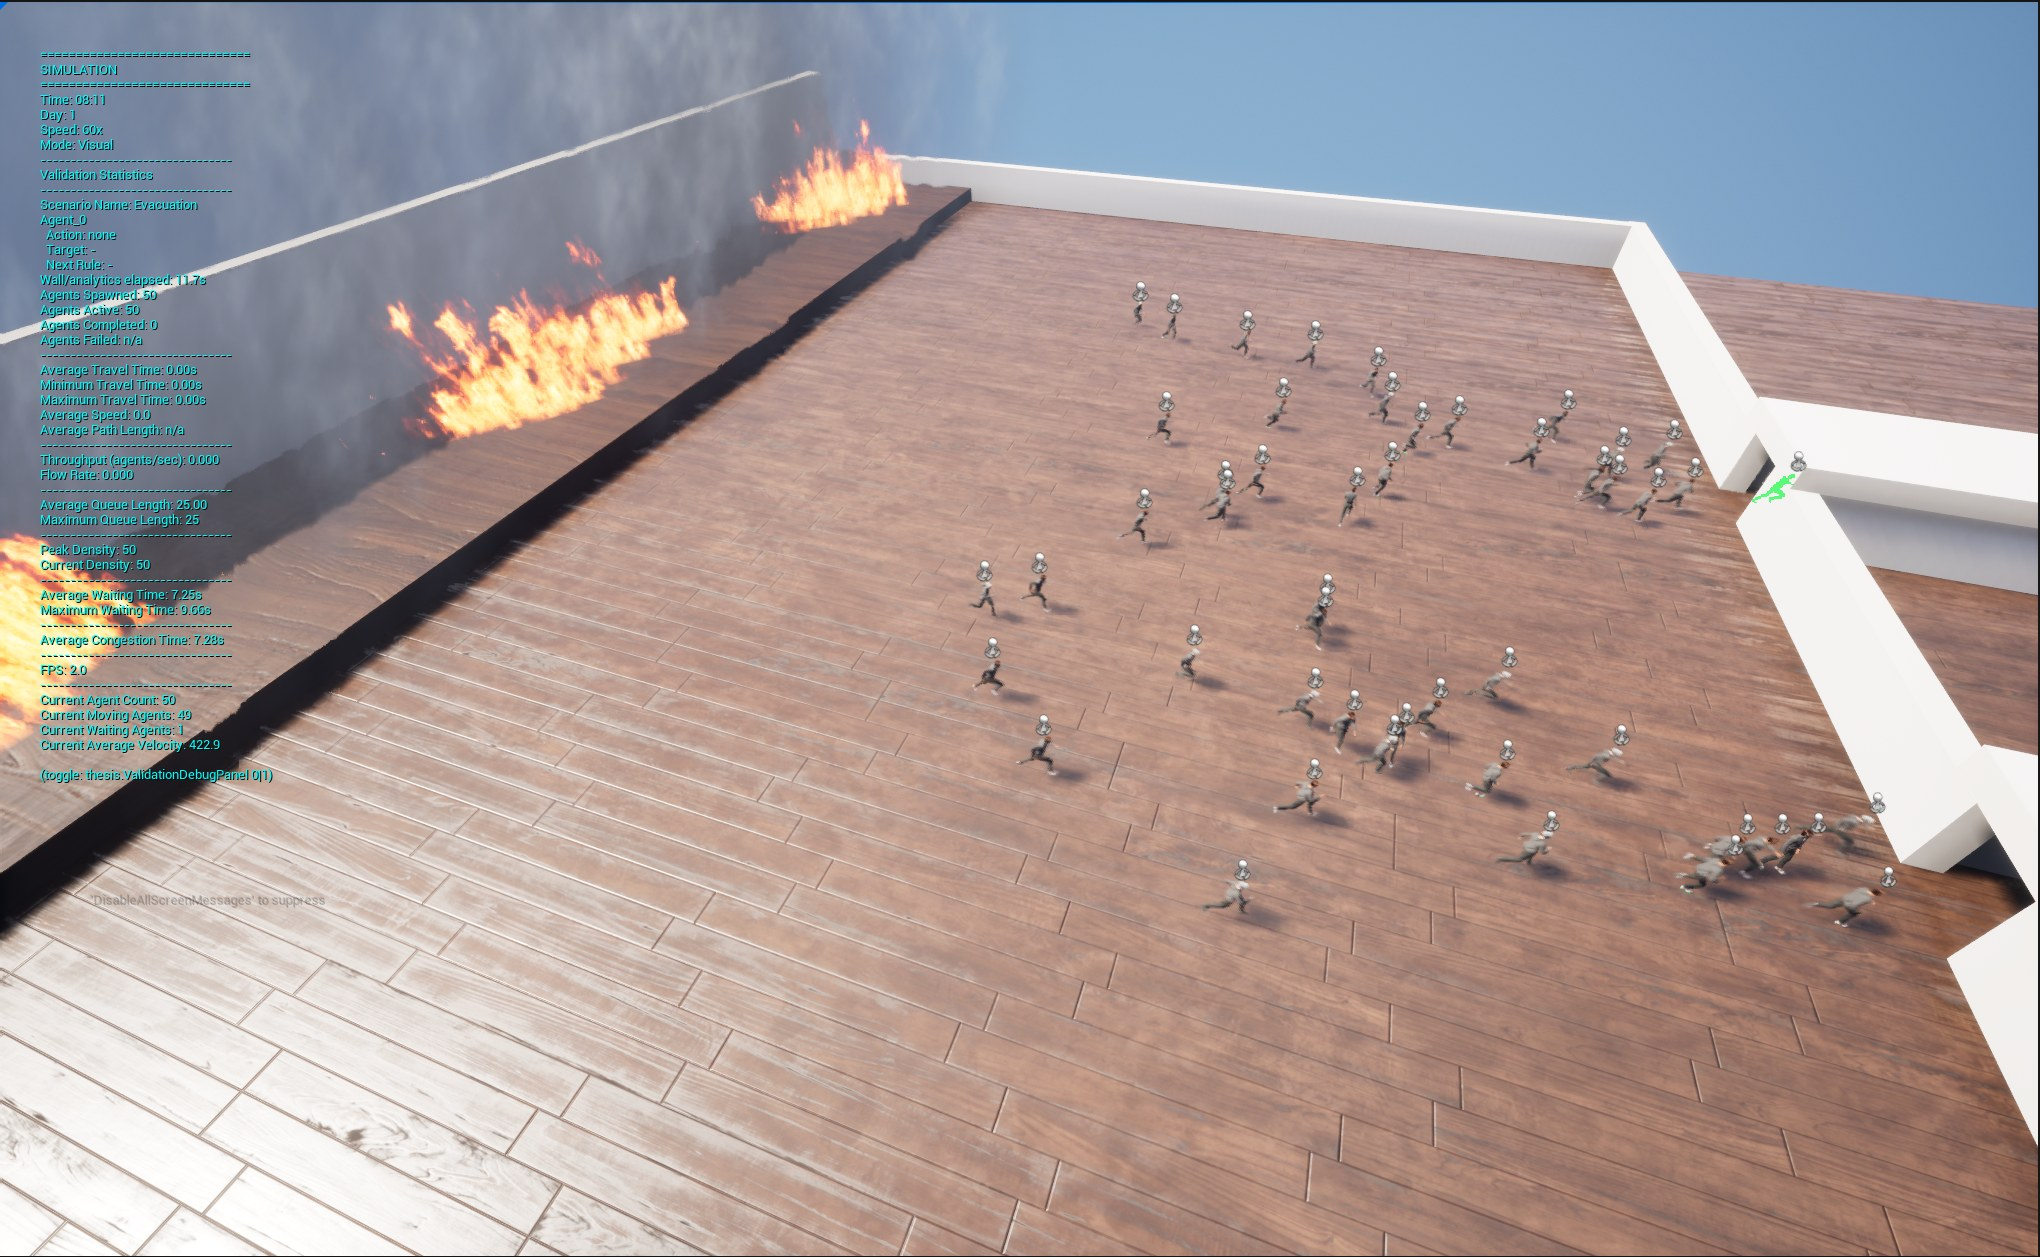
\includegraphics[width=0.85\textwidth]{images/shots/evac_exits.jpg}
\caption[Evacuation shortly after the alarm]{Evacuation shortly after the alarm, with the fire along one wall and the people heading for the exits.}
\label{fig:app-evac-exits}
\end{figure}

\begin{figure}[H]
\centering
\begin{tikzpicture}
\begin{axis}[
  width=0.85\textwidth, height=5.6cm,
  ybar=3pt, bar width=22pt, ymin=0, ymax=118,
  ytick={0,25,50,75,100},
  symbolic x coords={50,100,200}, xtick=data,
  xlabel={People}, ylabel={Passed an exit (\%)},
  axis lines=left, ymajorgrids, grid style={black!12},
  tick label style={font=\small}, label style={font=\small},
  /pgf/number format/assume math mode=true,
  enlarge x limits=0.25, legend image code/.code={\draw[#1] (0cm,-0.08cm) rectangle (0.3cm,0.14cm);},
  legend style={draw=none, fill=none, at={(0.5,1.02)}, anchor=south, legend columns=2, font=\small, /tikz/every even column/.append style={column sep=10pt}},
  nodes near coords, every node near coord/.append style={font=\scriptsize, inner sep=2pt, anchor=south, yshift=4pt, /pgf/number format/fixed, /pgf/number format/precision=0}]
\addplot[fill=cBlue, draw=cBlue!70!black, error bars/.cd, y dir=both, y explicit] table[x=agents, y=one, y error plus=one_hi, y error minus=one_lo] {analysis/data/evac_passed.dat};
\addlegendentry{1 s per frame}
\addplot[fill=cOrange, draw=cOrange!70!black, error bars/.cd, y dir=both, y explicit] table[x=agents, y=quarter, y error plus=quarter_hi, y error minus=quarter_lo] {analysis/data/evac_passed.dat};
\addlegendentry{0.25 s per frame}
\end{axis}
\end{tikzpicture}
\caption[People who passed an exit]{Share of people who passed an exit before the countdown ended (mean of three runs, error bars show the range), with every run in \cref{tab:res-evac-runs}.}
\label{fig:app-evac}
\end{figure}

\section{Directed-Flow Test Corridors}
\label{sec:app-validation}

Seven small maps test movement on their own: a corridor walked in one direction (V01) and in both (V02), a corner (V03), a bottleneck (V04), a T-junction (V05), a functional area whose twenty occupants all leave through one designated exit (V06) and two crossing diagonal flows (V07). Each map holds one or two cohorts written as super groups, whose members each receive a copy of the group's rules, and an on-screen panel reports flow, density, waiting and travel time. In the bottleneck map, for example, ten people idle for two minutes and then walk to \texttt{Exit\_Right}.

Each cohort walks to a single exit point with a 180~cm arrival radius, so runs finish with the cohort bunched around it, as at the work areas (\cref{fig:app-dul-arrivals}), and the panel's arrival counts depend on the target rather than on the corridor. Several panel measures are also proxies, as its density, for example, is the number of people on the map. We therefore used three of the seven maps for a single test of the hybrid blend, the one-way corridor, the two-way corridor and the bottleneck, because their straight flows make spread and speed easy to measure. The other four maps remain demonstrations of cohort rules.

\subsection{The hybrid blend on and off}
\label{sub:app-blend}

The blend is active in Accurate mode on scheduled walks, but not on walks to a reserved station, in a station queue or during the evacuation, so it shapes only part of the walking in this chapter, and here we isolate it. We ran the one-way corridor (V01), the two-way corridor (V02), and the bottleneck (V04) three times each with the blend and three times with \texttt{-NoBlend}, which leaves plain path following, and recorded every person's position once per simulated second (\cref{tab:app-blend}). The measures cover people still more than 6~m from their cohort's end point: the share of these position samples whose capsule (radius 34~cm) intersects another person's, the spread of each cohort across its direction of travel (the standard deviation of lateral positions), and its speed along that direction. The last columns give the time from a trip's start to within 4~m of the end point and the number of people who got there, where the end point is the cohort's centroid at its last sample rather than its target. Speed is sampled only more than 6~m from the end point and time covers the whole trip, so the two can disagree, as in the one-way corridor, where the blend lowered the speed but not the time to the end.

With the blend, the cohorts spread wider in the one-way corridor (154 against 144~cm) and in the bottleneck (128 against 103~cm), while in the two-way corridor the spread was about the same (120 against 123~cm), as were the arrivals (55 against 57 of 60). In the bottleneck, the cohorts also reached their end point sooner (37 against 45~s), and more people got there (57 against 53 of 60). Overlaps were rare in every setting, at most 3\% of position samples in any run. Samples are one simulated second apart, so short overlaps between samples are missed. With three runs per setting, and with corridor runs that a seed does not reproduce (\cref{sub:res-same-seed}), these are directions, not sizes: the blend spread the cohorts in two of the three maps and helped where people converge, and it does not prevent overlaps.

\begin{table}[H]
\centering
\small
\begin{tabular}{|l|l|c|c|c|c|c|}
\hline
\rowcolor{headgray}\textbf{Map} & \textbf{Blend} & \textbf{\shortstack{Overlapping\\samples (\%)}} & \textbf{\shortstack{Spread\\(cm)}} & \textbf{\shortstack{Speed\\(cm/s)}} & \textbf{\shortstack{Time to\\end (s)}} & \textbf{\shortstack{People that\\got there}} \\
\hline
\tabinput{analysis/tables/blend_rows.tex}
\end{tabular}
\caption[Hybrid blend on and off]{Hybrid blend on and off in three test maps with three runs each, where overlaps show the mean with the range over runs in parentheses, spread is measured across the direction of travel and speed along it, as the median over runs.}
\label{tab:app-blend}
\end{table}

\section{Performance and System Scalability on One Machine}
\label{sec:app-performance}

We raised the population of the evacuation and of Daily Urban Life from 50 to 1600 people. The stress-test subsystem copies the level's people at start, and in Daily Urban Life, each copy received the rules of one of the 50 original people, so homes and desks were shared by more people as the population grew. After 30 seconds of warm-up, it recorded 120 seconds of frames in Visual mode, the mode for watching (\cref{sub:app-settings}), with vertical synchronization off, twice per population up to 400 people and once at 800 and 1600 (\cref{fig:app-scaling}).

Taking 30 frames per second as a common interactive threshold, the evacuation stayed above it on average with 100 people (32.8), although its 95th-percentile frame times of 51.4 and 47.0~ms correspond to 19 to 21 frames per second. Daily Urban Life reached the threshold with 50 people (37.6) but not with 100 (16.9). Between 50 and 800 people, the frame time grows roughly in proportion to the population in the evacuation and faster than that in Daily Urban Life, with fitted exponents of about 0.9 and 1.2 on logarithmic axes. The limit is the update of the people on the processor, as in every run the game-thread time equaled the frame time to within rounding. Between 50 and 800 people, the render thread needed 3.9 to 43.6~ms on average, at most a quarter of the frame time (in Daily Urban Life with 50 people), and the \gls{gpu} needed at most 40.6~ms per frame on average, in Daily Urban Life with 800 people (\cref{tab:res-scaling-runs}). Neighbor queries, boids forces, sonar and wall probes and synchronous path queries all run on the game thread. The faster growth in Daily Urban Life is consistent with its shared destinations putting more neighbors around each moving person as the population grows, although we did not confirm the cause with a profiler. Each character also has a fixed cost, as after the evacuation countdown, when no person moves, a frame still took 0.17 to 0.22~ms per person. Below 30 frames per second, a rendered run in Accurate mode covers more than one simulated second per frame, which can change its results (\cref{sub:app-step}), so the batch runs used the fixed step.

\begin{figure}[H]
\centering
\begin{tikzpicture}
\begin{groupplot}[
  group style={group size=2 by 1, horizontal sep=1.6cm},
  width=0.48\textwidth, height=5.6cm,
  xmode=log, log basis x=2, xtick={50,100,200,400,800,1600}, xticklabels={50,100,200,400,800,1600},
  xlabel={People}, axis lines=left, ymajorgrids, grid style={black!12},   tick label style={font=\small}, label style={font=\small},   /pgf/number format/assume math mode=true,
  legend style={draw=none, fill=none, font=\footnotesize}, legend cell align=left]
\nextgroupplot[ymode=log, ymin=0.35, ytick={0.5,1,2,5,10,30,60}, yticklabels={0.5,1,2,5,10,30,60}, ylabel={Frames per second}, legend style={at={(0.98,0.98)}, anchor=north east}]
\addplot[cBlue, mark=*, mark size=1.6pt, line width=0.8pt, unbounded coords=jump] table[x=agents, y=evac_fps] {analysis/data/scaling_fps.dat};
\addlegendentry{Evacuation}
\addplot[cVerm, dashed, mark=square*, mark size=1.6pt, line width=0.8pt] table[x=agents, y=dul_fps] {analysis/data/scaling_fps.dat};
\addlegendentry{Daily Urban Life}
\addplot[black!70, densely dashed, thin, forget plot, domain=50:1600, samples=2] {30};
\nextgroupplot[ymin=0, ymax=17, ylabel={Peak memory used (GB)}, legend style={at={(0.02,0.98)}, anchor=north west}]
\addplot[cBlue, mark=*, mark size=1.6pt, line width=0.8pt, unbounded coords=jump] table[x=agents, y=evac_gb] {analysis/data/scaling_fps.dat};
\addlegendentry{Evacuation}
\addplot[cVerm, dashed, mark=square*, mark size=1.6pt, line width=0.8pt] table[x=agents, y=dul_gb] {analysis/data/scaling_fps.dat};
\addlegendentry{Daily Urban Life}
\end{groupplot}
\end{tikzpicture}
\caption[Frame rate and memory by number of people]{Frame rate (left) and peak memory (right) by number of people in Visual mode, where the dashed line marks 30 frames per second and the Daily Urban Life point at 1600 people is not comparable with the others, while the evacuation has no point there because it crashed in its first frame (every run in \cref{tab:res-scaling-runs}).}
\label{fig:app-scaling}
\end{figure}

We repeated each population once with \texttt{-StressHideMeshes}, which hides the MetaHuman meshes and stops their animation and hair, to separate the framework from the characters (\cref{tab:app-nomesh}). In the evacuation, the characters took 49 to 67\% of the frame time, and without them, a frame took 12.7~ms with 100 people and 33.8~ms with 400. In Daily Urban Life, they took only 16 to 34\%, and the framework alone needed 19.0~ms for 50 people and 38.8~ms for 100. The people's own update, with neighbor queries and synchronous path queries at shared destinations, is the limit.

\begin{table}[H]
\centering
\small
\begin{tabular}{|l|r|c|c|c|}
\hline
\rowcolor{headgray}\textbf{Scenario} & \textbf{People} & \textbf{\shortstack{Characters\\shown (ms)}} & \textbf{\shortstack{Characters\\hidden (ms)}} & \textbf{\shortstack{Frame time spent\\on characters (\%)}} \\
\hline
\tabinput{analysis/tables/nomesh_rows.tex}
\end{tabular}
\caption[Frame time with and without the characters]{Mean frame time with the MetaHuman characters shown and hidden, and the share of the frame time that the characters took.}
\label{tab:app-nomesh}
\end{table}

The cost also changes during a run (\cref{fig:app-phase}), as with 400 people, the evacuation reached its lowest frame rate about 15 seconds in, when all people chose exits and planned paths at once, and recovered when the countdown ended. Daily Urban Life, in contrast, slowed steadily as more people set off.

\begin{figure}[H]
\centering
\begin{tikzpicture}
\begin{axis}[
  width=0.9\textwidth, height=5.5cm,
  xmin=0, xmax=150, ymin=0, ymax=18,
  xtick={0,20,...,140}, ytick={0,5,10,15},
  xlabel={Real seconds since the run started}, ylabel={Frames per second},
  axis lines=left, ymajorgrids, grid style={black!12},
  tick label style={font=\small}, label style={font=\small},
  /pgf/number format/assume math mode=true,
  legend style={draw=none, fill=none, at={(0.02,0.98)}, anchor=north west, font=\small}, legend cell align=left]
\addplot[cBlue, line width=0.9pt] table[x=t, y expr=1000/\thisrow{frame}] {analysis/data/phase_evac_400.dat};
\addlegendentry{Evacuation, 400 people}
\addplot[cVerm, dashed, line width=0.9pt] table[x=t, y expr=1000/\thisrow{frame}] {analysis/data/phase_dul_400.dat};
\addlegendentry{Daily Urban Life, 400 people}
\draw[->, >=Latex, black!60] (axis cs:15,2.2) -- (axis cs:15,3.75);
\node[font=\footnotesize, anchor=north west, inner sep=1pt, text=black!75] at (axis cs:11,2.2) {people choose exits};
\node[font=\footnotesize, anchor=south, inner sep=2pt, text=black!75] at (axis cs:134,15.7) {countdown ends};
\end{axis}
\end{tikzpicture}
\caption[Frame rate during one run with 400 people]{Frame rate during one run of each scenario with 400 people (5-second bins).}
\label{fig:app-phase}
\end{figure}

Between 50 and 800 people, memory grew by about 7.4~MB per person in the evacuation and 7.3~MB in Daily Urban Life, from about 2.6~GB and 3.6~GB, so the 32~GB of the machine was not the limit. The evacuation with 1600 people crashed in its first frame with an assertion in the engine's render graph and the hair-strands module in the call stack. Daily Urban Life ran with 1600 people at 0.44 frames per second, and at such rates the clock falls behind real time and movement takes large steps, so behavior at the largest populations is not comparable with the smaller ones.

\section{Threats to Validity}
\label{sec:app-threats}

With the fixed time step, a seed reproduced a run exactly in the Mall A pairs we compared, but not in the corridors or in Daily Urban Life (\cref{sub:res-same-seed}). Mall A runs with the same seed label under different settings therefore share their random draws until the settings make them diverge, while the tests treat runs as independent samples, which is conservative, since a paired test over seed labels would have more power. Because these runs differ so little, a low $p$-value marks a consistent direction rather than a large effect, as the tables show with about 20 seconds per visit. The measures are proxies defined by our implementation: the wait per visit ignores the time a place is held while its owner walks, late minutes are attributed with a fixed precedence and stop at dispatch, and arrival counts are an upper bound, because a walk counts as arrived whenever the walk action completes. The results depend on the frame step (\cref{sub:app-step}), as movement within a frame of one simulated second is coarse, while with 0.25 seconds, more walks stalled and an unreleased reservation dominated one counter run. The edge cases of \cref{sub:app-edge-cases} dominate some runs, and the GoTo time-out and the exit service, which count real seconds, lengthen some Daily Urban Life walks and slow every exit of the evacuation. People walk faster than free pedestrians, the scaling runs were measured in Visual mode rather than in rendered Accurate mode, only three of the seven corridor maps were measured, and larger populations were obtained by copying people. All performance results come from one machine, a Development editor build and one set of MetaHuman characters, and the runs without characters (\cref{tab:app-nomesh}) are single runs, so the character shares are estimates. No run was compared with observed pedestrians, so a reduction in simulated waiting describes the model, not a real building.

\subsection{Edge cases and their effect on each result}
\label{sub:app-edge-cases}

The runs exposed five edge cases of the implementation, and \cref{tab:app-edge-cases} states for each one which runs it affects and whether it changes the direction of a result or only its size.

The direction of every capacity result, and the medians that report it, survive these cases, but the mean with three counter places does not, so its median of 1.26 minutes is the value to use. The same holds in the lunch rush, where one undiagnosed run with three counter places averaged 31.5 minutes.

\begin{table}[H]
\centering
\footnotesize\renewcommand{\arraystretch}{1.15}
\begin{tabularx}{\textwidth}{|L{4.2cm}|L{3.6cm}|>{\raggedright\arraybackslash}X|}
\hline
\rowcolor{headgray}\textbf{Edge case} & \textbf{Runs it affects} & \textbf{What it changes} \\
\hline
A reservation has no time-out, so an admitted person who never reaches the place holds it & 3 of the 30 Mall A runs with three counter places, and one counter run at 0.25~s per frame & The mean wait with three counter places (2.43 minutes, against 1.25 in the other 27 runs), but not its median (1.26) or the direction of any capacity result \\ \hline
A queue stays bound to the first matching station & Every Mall A run with a queue, including the lunch rush & Which station queues and the size of the waits, while the direction held in every comparison \\ \hline
Walks end at single target points, and a person who cannot settle there ends their walk only at the GoTo time-out & Daily Urban Life, one diner in every lunch-rush run, and the Mall A runs with copied people & The mean walk to a work area (7.5 minutes, 5.0 without the 7 time-out walks) and the size of the mall populations, which jammed when copied \\ \hline
Exit queues can stall & Evacuation runs with 100 and 200 people & How many people passed an exit (89 to 100 of 100 and 44 to 75 of 200 at one-second steps) \\ \hline
The first arrivals block the rim of the safe zone & Every evacuation run & The number counted as safe (10 to 31 per run), so we report passing an exit instead of casualties \\ \hline
\end{tabularx}
\caption[Edge cases and their effect on each result]{Edge cases of the implementation and the results they change.}
\label{tab:app-edge-cases}
\end{table}

\subsection{Frame step}
\label{sub:app-step}

Every behavioral result above uses one simulated second per frame, so we repeated the counter tests with one and three places (five seeds each), two Daily Urban Life runs and the evacuation with 0.25 simulated seconds per frame (\texttt{analysis/step\_check.py}). The evacuation improved with the finer step (\cref{sub:app-evac-results}), while in Daily Urban Life fewer rules were carried out (564 against 591 of 608 in the two runs, with 44 against 17 dropped as overdue). Fewer walks also arrived (171 against 187 of 200), fewer station visits ended in a completed service (92 against 127), and 29 walks failed, against 13. In Mall A, every rule was dispatched at both steps in all but one run, but one or two exit walks per run had not arrived when the run ended, 21 in the ten runs against 1 at one-second steps. With one counter place, the mean wait per visit rose from 0.81 to 1.16 simulated minutes (median 0.84 at both steps). With three places, it rose from 1.35 to 2.90, mostly because of one seed with the reservation edge case of \cref{sub:app-edge-cases}. The direction of the counter result held at both steps, but its size did not, and with only two step sizes we cannot say whether the results converge at finer steps.

\section{Summary}
\label{sec:app-summary}

One implementation of a person ran every scenario of this chapter with only one new action, \texttt{Interact}, and queueing was 76\% of the start delay of station rules in Mall A as authored and 92\% in a lunch rush with one counter place, while long walks to crowded target points took most of the delay in Daily Urban Life. Extra places helped only at the stage of a pipeline that was short of capacity, a direction that held at both frame steps and survives the edge cases of \cref{sub:app-edge-cases}.
